\NeedsTeXFormat{LaTeX2e}[1995/12/01]
\documentclass[10pt]{bmc_article}


% Load packages
%\usepackage{hyperref}
\usepackage{cite} % Make references as [1-4], not [1,2,3,4]
\usepackage{url} % Formatting web addresses
\usepackage{ifthen} % Conditional
\usepackage{multicol} %Columns
\usepackage{xspace}
\usepackage[utf8]{inputenc} %unicode support
%\usepackage[applemac]{inputenc} %applemac support if unicode package fails
%\usepackage[latin1]{inputenc} %UNIX support if unicode package fails
\urlstyle{rm}
\usepackage[OT1]{fontenc} 

\usepackage{rotating}
\usepackage{colortbl}
\usepackage{color}
\usepackage{comment}

\usepackage{subfigure}

\newcommand {\pg}[1]{\textcolor{blue}{#1}}
\newcommand {\ppg}[1]{\textcolor{blue}{#1}}
\newcommand {\new}[1]{\textcolor{green}{#1}}

\newcommand{\minitab}[2][l]{\begin{tabular}{#1}#2\end{tabular}}


%\newcommand{} {\mbox{}\xspace}

\def\squeezetable{\def\tabular@font{\tiny}}%

% Change useable area of a page to be slightly larger
\setlength{\topmargin}{0.0cm}
\setlength{\textheight}{21.5cm}
\setlength{\oddsidemargin}{0cm}
\setlength{\textwidth}{16.5cm}
\setlength{\columnsep}{0.6cm}

\newboolean{publ}

%Settings: comment\uncomment bmcformat definition to get format required

%Review style settings
\newenvironment{bmcformat}{\begin{raggedright}\baselineskip20pt\sloppy\setboolean{publ}{false}}{\end{raggedright}\baselineskip20pt\sloppy}

%Publication style settings
%\newenvironment{bmcformat}{\fussy\setboolean{publ}{true}}{\fussy}


% Begin ...
\begin{document}
\begin{bmcformat}

\title{Supplementary material for: non-coding RNAs of bird genomes}

\author{
Paul P. Gardner\correspondingauthor$^{1,2}$
\email{Paul P. Gardner\correspondingauthor - paul.gardner@canterbury.ac.nz},
Mario Fasold$^5$
\email{mario@bierdepot.bioinf.uni-leipzig.de},
Sarah W. Burge$^3$
\email{sb30@sanger.ac.uk},
Jana Hertel$^5$
\email{Jana Hertel\correspondingauthor - jana@bioinf.uni-leipzig.de},
Maria Ninova$^4$
\email{Maria.Ninova@postgrad.manchester.ac.uk},
Stephanie Kehr$^5$
\email{steffi@bierdepot.bioinf.uni-leipzig.de},
Tammy E. Steeves$^1$
\email{tammy.steeves@canterbury.ac.nz},
Sam Griffiths-Jones$^4$
\email{sam.griffiths-jones@manchester.ac.uk}
and
Peter Stadler\correspondingauthor$^5$
\email{Peter Stadler\correspondingauthor - studla@bioinf.uni-leipzig.de}
}
\address{
\iid(1) School of Biological Sciences, University of Canterbury, Private Bag 4800, Christchurch, New Zealand.
\iid(2) Biomolecular Interaction Centre, University of Canterbury, Private Bag 4800, Christchurch, New Zealand.
\iid(3) European Molecular Biology Laboratory, European Bioinformatics Institute, Hinxton, Cambridge, CB10 1SD, UK.
\iid(4) Faculty of Life Sciences, University of Manchester, Manchester, United Kingdom.
\iid(5) Bioinformatics Group, Department of Computer Science; and Interdisciplinary Center for Bioinformatics, University of Leipzig, H{\"a}rtelstrasse 16-18, D-04107 Leipzig, Germany
}

\maketitle

%\begin{abstract}
%...
%\end{abstract}


\ifthenelse{\boolean{publ}}{\begin{multicols}{2}}{}

%\section*{Supplementary introduction}
%...

\section*{Supplementary results}

In the following we explore in further detail the results that were
not discussed in the main manuscript. 

\subsection*{Classic RNAs: LUCA and LECA}

Many RNA families constitute the most evolutionarily conserved genes
across all life on this planet \cite{Jeffares:1998}. Examples of RNAs
derived from the Last Universal Common Ancestor (LUCA) include, the
transfer RNAs (tRNA), ribosomal RNAs (rRNA), RNA components of RNase P
(RNase P RNA), RNase MRP (RNase MRP RNA) and the signal recognition
particle (SRP RNA). Other classes of RNA are likely to have been
components of the Last Eukaryotic Common Ancestor (LECA) include the
telomerase RNA, major spliceosomal RNAs (U1, U2, U4, U5, and U6) and
the minor spliceosomal RNAs (U11, U12, U4atac, and U6atac)
\cite{Hoeppner:2012}.

Unsurprisingly, the bulk of these classes of RNAs are well represented
across the bird genomes (See Figure~\ref{fig:1}). However, there
appear to have been ``losses'' of a few of these RNAs in certain bird
species. Some of these may be due to sequence divergence, of which
there are several notable examples e.g.
\cite{Leonardi:2008,Webb:2008,Mao:,Lai:2010,Chan:2011}. Other losses
may be due to incomplete genome coverage.

A number of the classic RNAs are incorporated into RNA-protein
complexes (RNPs) involved in core cellular processes. An example of
this are the spliceosomal RNAs. Based upon the presence/absence
patterns of the major spliceosomal RNAs they are all well represented
in these genome sequences. The exceptions to this observation are the
U4 RNA in cormorant and the U5 RNA in the bee eater which are both
missing. These two genomes are low coverage, suggesting these
genes weren't captured in the current assembly. The minor spliceosomal
RNAs are more interesting, the U4atac and U11 snRNAs show widespread
patterns of loss, even in some of the high coverage genomes. These
RNAs are frequently missed in bioinformatic screens. Indicating either
frequent loss \cite{Davila_Lopez:2008} or sequences that have diverged
beyond the ability of detection by covariance models \cite{Marz:2008}.

The telomerase RNA is also largely missing from the avian
annotations. This RNA acts as a template for the telomerase enzyme
that extends the telomeres found on chromosome ends. It is only found
in the chicken, bald eagle, kea, budgerigar, crow and
zebrafinch. Homology searches searches with the telomerase reverse
transcriptase (TERT) protein show that the protein component of the
telomerase RNP is conserved across all the bird genomes (data not
shown). This pattern of presumably divergent telomerase RNA and
conserved telomerase protein has been noted previously, most notably
in the fungi \cite{Leonardi:2008,Webb:2008}.

The the RNA components of RNase P and RNase MRP also appear to have
undergone dramatic losses within the bird lineage. RNase P is required
for the maturation of tRNA, the paralogous enzyme, RNase MRP is
required for the maturation of rRNA. Each RNP cleaves smaller RNAs
from larger transcripts \cite{Lopez:2009}. It is unlikely that the
these genes have been lost in any of the birds. Homology searches with
the RNase associated protein coding genes (POP1, POP4, POP5, POP7,
RPP1, RPP14, RPP25, RPP38, RPP40 and RPR2), identified viable homologs
of each in all of the bird genomes \cite{Rosenblad:2006} (data not
shown). This suggests that the bird RNase P and MRP RNAs may have
diverged slightly from the canonical models.

The 5.8 S component of the ribosome in the turtle, turkey bustard,
hoatzin, flamingo, tropicbird, seriema, owl, cuckoo roller, trogon,
bee eater and falcon appears to have been lost (See
Figure~\ref{fig:1}). The rRNA repeats are frequently not assembled,
consequently it is not surprising to see ``losses'' in these \cite{Floutsakou:2013}.
Furthermore, the genomes for these species are also
low-coverage.


\subsection*{Small nucleolar RNAs}

Small nucleolar RNAs (snoRNAs) are important ncRNAs that participate
in the maturation of other functional RNAs \cite{Gardner:2010}. The
bulk of the characterised snoRNAs guide either methylation or
pseudouridylation modifications, primarily of rRNAs but also
spliceosomal RNAs. The two types of modifications are guided by two
different types of RNA, the box C/D and the H/ACA snoRNAs
respectively, each with a characteristic cohort of motifs and
secondary structures \cite{Marz:2011}.

There are 66 ribosomal modification sites, guided by 59 snoRNA
families, that are preserved between \emph{H. sapiens} and
\emph{S. cerevisiae} \cite{Lestrade:2006}. Of these, 45 snoRNA
families are conserved in the bird dataset.
Over a third of the apparent losses of the yeast-human conserved
snoRNA families appear to cluster on 2 loci of the ancestral
vertebrate genome. We investigated these losses further.

The first cluster is found at chr11:62620797-62622484 on the human
genome (hg19) and contains SNORD27, SNORD29 and SNORD31 of the
human-yeast conserved snoRNAs. These snoRNAs are located in the
inside-out gene SNHG1 which hosts a total of eight C/D box snoRNAs:
SNORD25, SNORD26, SNORD27, SNORD28, SNORD29, SNORD22, SNORD30 and
SNORD31 \cite{Tycowski:1996}. Each of which are also found in the
alligator and turtle genomes within a 3-4 KB locus, yet these have
largely been lost in the birds. Notable exceptions are five of the
eight are located in the tinamou genome, these are located on the same
scaffold and are within 2 KB of each other. This implies that SNHG1 is
conserved in the tinamou. Loci with four of the eight snoRNAs can be
found in zebrafinch, ground-finch, and bald eagle. Still, three of the
eight are located in the ostrich, crow, and cockoo genomes, again
within 2 KB of each other on the same scaffolds. This complex pattern
of loss could be attributed to many different models, e.g. multiple
losses in birds, poor homology modelling or incomplete genome
sequences.


The second cluster is located at chr19:49993222-49994231 on the human
genome (hg19) and contains two copies of SNORD33 and one SNORD34 all
within a 1 KB genomic region. The turtle and alligator genomes retain
the two copies of SNORD33 yet don't have an obvious SNORD34 gene on
the same scaffold. Within the bird genomes, the crow and rifleman each
retain a single SNORD33 and SNORD34 gene on the same scaffold. While
the ground-finch and bald eagle retain a single SNORD33 and the
zebrafinch and seriema retain a single SNORD34 (See
Figure~\ref{fig:3}).  In human these snoRNAs are intronic to the host
gene, ribosomal protein L13a (RPL13A). Based on BLASTP (version
2.2.18) homology searches for the RPL13A gene, the protein is
conserved in the human and turtle genomes and in the bald eagle, crow,
rifleman and zebrafinch avian genomes (data not shown). Therefore the
conservation patterns of the RPL13A host gene and corresponding
intronic snoRNAs largely mimic each other, each independently supports
a pattern of loss of the RPL13A gene and the intronic snoRNAs that it
hosts in the bird genomes.


\subsection*{MicroRNAs}
MicroRNAs are an important class of non-coding RNA. They have been
found in the genomes of Chromalveolata \cite{Cock:2010,Huang:2011},
Metazoa \cite{Lee:1993,Lau:2001,Hertel:2006}, Mycetozoa
\cite{Hinas:2007,Avesson:2012}, Viridiplantae
\cite{Reinhart:2002,Fattash:2007,Axtell:2007,Molnar:2007} and Viruses
\cite{Pfeffer:2004,Ouellet:2008,Pfeffer:2005,Landgraf:2007}. The
miRNAs have been shown to regulate the expression of large numbers of
messenger RNAs \cite{Lim:2005}. The mature miRNA product is generally
22 nucleotides long which is usually processed from a larger RNA that
is characterised by a stable hairpin-shaped secondary structure.

Chicken and zebrafinch are the only birds with previously annotated
microRNAs. We searched for homologs of these and other vertebrate
microRNAs in the genomes of the 48 birds, American alligator and green
turtle. Overall, we annotate a total of 16617 putative microRNA loci,
homologous to 543 known microRNA genes, of which 487 are annotated in
chicken and/or zebra finch, while 56 have been so far known only in
non-avian vertebrates. The numbers of annotated loci in the individual
species are approximately equal - 300-400 per species, except for the
turkey (Meleagris gallopavo) where we identified 543 sequences
homologous to known microRNAs.

In addition, we can confidently identify a further 3 microRNA
families that are present in mammals, and turtle and/or crocodile, but
not in any avian genome (mir-150, mir-208, mir-590). This suggests
that these sequences were lost in the last common ancestor of
archosaurs or birds. There are also a number of microRNAs that are
predicted to be present in turtles and/or crocodiles, and only a small
number of bird genomes. Indeed, there are many missing annotations,
species-specific and otherwise, that are not consistent with the
consensus phylogeny, and could be due to either incomplete genomes or
widespread microRNA loss.

The turkey genome contains a high number (190) of microRNAs so far
found only in chicken, which account for the higher number of
annotated sequences in this genome compared with other birds. This is
consistent with its phylogenetic position as the closest chicken
relative among the examined birds. However, 101 chicken microRNAs
have no homolog in the turkey or other bird genomes, suggesting that
these genes are chicken-specific. This is consistent with previous
reports of large number of speciesspecific microRNAs in all animals,
and supports the view of fast microRNA turnover during animal
evolution.



\subsection*{Cis-regulatory elements}
%% Histone3, IRE, IRES, K chan RES, SECIS, Antizyme FSE, Vimentin3, GABA3,
%% CAESAR,

The cis-regulatory RNAs are a group of RNA structures encoded on
mRNAs. Generally they are involved in regulating the expression of the
mRNA they are encoded within. Others may recode the translated protein
product into an alternate sequence.

This group includes the iron response element (IRE) \cite{Stevens:}
and the histone $3^\prime$ UTR (histone3)
\cite{Davila_Lopez:2008a}. These are structured motifs bound by
regulatory proteins. The selenocysteine insertion sequence (SECIS) is
a structured motif that recodes UGA stop codons to selenocysteines
\cite{Lambert:2002} and the GABRA3 stem-loop is a structure recognised
by the ADAR enzyme family. This enzyme edits adenine nucleotides to
inosine, in this case recoding an isoleucine codon to methionine in
exon 9 of the GABRA3 gene \cite{Ohlson:2007}.

These regulatory elements and others, including an internal ribosome
entry site (IRES), potassium channel RNA editing signal (K chan RES),
Antizyme RNA frameshifting stimulation element (Antizyme FSE),
vimentin $3^\prime$ UTR protein-binding region (Vimentin3) and a
connective tissue growth factor (CTGF) $3^\prime$ UTR element (CAESAR)
are conserved across a diverse group of vertebrates, including the
bird lineages explored here (See Figure~\ref{fig:1}).

\subsection*{Unexpectedly poorly conserved  ncRNAs: testing divergence}

In order to get an idea to what extent the
absence of these RNAs from the \texttt{infernal-based} annotation is
caused by sequence divergence beyond the thresholds of the Rfam CMs
and/or missing or incomplete data, we complemented our analysis by
dedicated searches for a few of these RNA groups.

The simplest case are the selenocysteine tRNAs. Here, tRNAscan is
tuned for specificity and thus misses several occurrances that are
easily found by \texttt{blastn} with $E\le 10^{-30}$. In some cases
the sequences appear degraded at the ends, which may be explained
e.g.\ by low sequence quality at the very ends of contigs or
scaffolds. A \texttt{blastn} search also readily retrieves additional
RNase P and RNAse MRP RNAs, capturing only the best conserved
regions. In many cases these additional candidates are incomplete or
contain undetermined sequence, explaining why they are missed by the
CMs. Overall, we identify tRNA-Sec in most and RNAse P and MRP RNAs in
the majority of the genomes. An additional candidate could also be
retrieved for telomerase RNA. Telomerase is well known to exhibit very
poor sequence conservation and rapid variations in size that make it
notoriously hard to identify by homology search \cite{Xie:08a}. The
poor return thus does not come as a surprise. Vault RNA homology
searches with \texttt{blastn} remained unsuccessful, therefore we
constructed a sauropsid-specific CM.  In addition to the hits
identified by the Rfam model we obtained three additional
homologs. Vault RNAs, with a size of about 100 nt, exhibit conserved
sequence patterns only at their ends, with essentially unconstrained
sequence in the central part. Their identification is one of the
well-known and difficult problems for homology search
\cite{Stadler:09b,Kolbe:2009}.

Our ability to find additional homologs for several RNA families that fill
gaps in the abundance matrices (Figure~\ref{fig:2})
strongly suggests that conspicuous absences, in particular of LUCA and
LECA RNAs, are caused by incomplete data in the current assemblies and
sequence divergence rather then true losses.



 \begin{figure}[ht]
   \includegraphics[width=0.95\textwidth]{figures/figure2.pdf}
\caption{Additional homologs of some sparsely represented RNA families were
discovered using dedicated search strategies combined with highly
sensitive settings, synteny information, lineage-specific CMs and
subsequent manual inspection.}\label{fig:2}
 \end{figure}


\subsection*{Exceptional RNAs}

%Background to this group...

A number of other ncRNAs can also be found in Eukaryotic
genomes. These do not fit into the main classes of RNA but still
perform vital roles in the function and evolution of Eukaryotes.
Their functions are diverse and many have not yet been characterised.

An example of an uncharacterised RNA is the ultraconserved element,
uc.338 (also known as TUC338)
\cite{Bejerano:2004,Bejerano:2006,Braconi:2011}. The uc.338 element
is derived from a short interspersed element (SINE) called the
lobe-finned fishes SINE (LF-SINE) as it is conserved between the
coelacanth and mammals \cite{Bejerano:2006}. Analysis of the
expression of uc.338 implies that it plays a role in the progression
of hepatocellular carcinoma, possibly by influencing cell growth
\cite{Braconi:2011}. This RNA is conserved in the birds and appears to
have been duplicated in several lineages.

The Y RNA is an enigmatic ncRNA where we know very little about the
function. It was discovered in the 1980s in ribonucleoprotein
complexes \cite{Lerner:1981}. The function of the Y RNAs remain
unknown, but evidence is emerging that they may be associated with DNA
replication \cite{Christov:2006}. There are 4 functional Y RNAs
encoded in the human genome, Y1, Y3, Y4 and Y5. However, there are
hundreds of pseudogenised copies of the Y RNA scattered throughout the
human genome \cite{Mosig:2007}. In the birds and other lizards, we
identify between two and seven Y RNA paralogs (See
Figure~\ref{fig:1}).

The Vault RNA forms a major component of the vault ribonucleoprotein
complex, this is one of the largest particles found in the vertebrate
cell; In fact, it is larger than the ribosome \cite{Kong:1999}. As yet
not much is known about the function of Vault. The Vault RNA has been
shown to be broadly conserved in metazoans
\cite{Stadler:2009}. However, in the bird lineages it appears to have
either been lost or diversified.


\subsection*{Contamination}

Bacterial families can be used to identify problematic sequences that
are likely to be the result of contamination from non-avian
sources. We identified a number of RNA families of bacterial origin in
the avian genomes. These have been reported and will be dealt with in
later updates to the avian genome sequences.

%{\bf WRITE MORE HERE!}


%%%%%%%%%%%

\clearpage
\newpage

\begin{figure}[ht]
  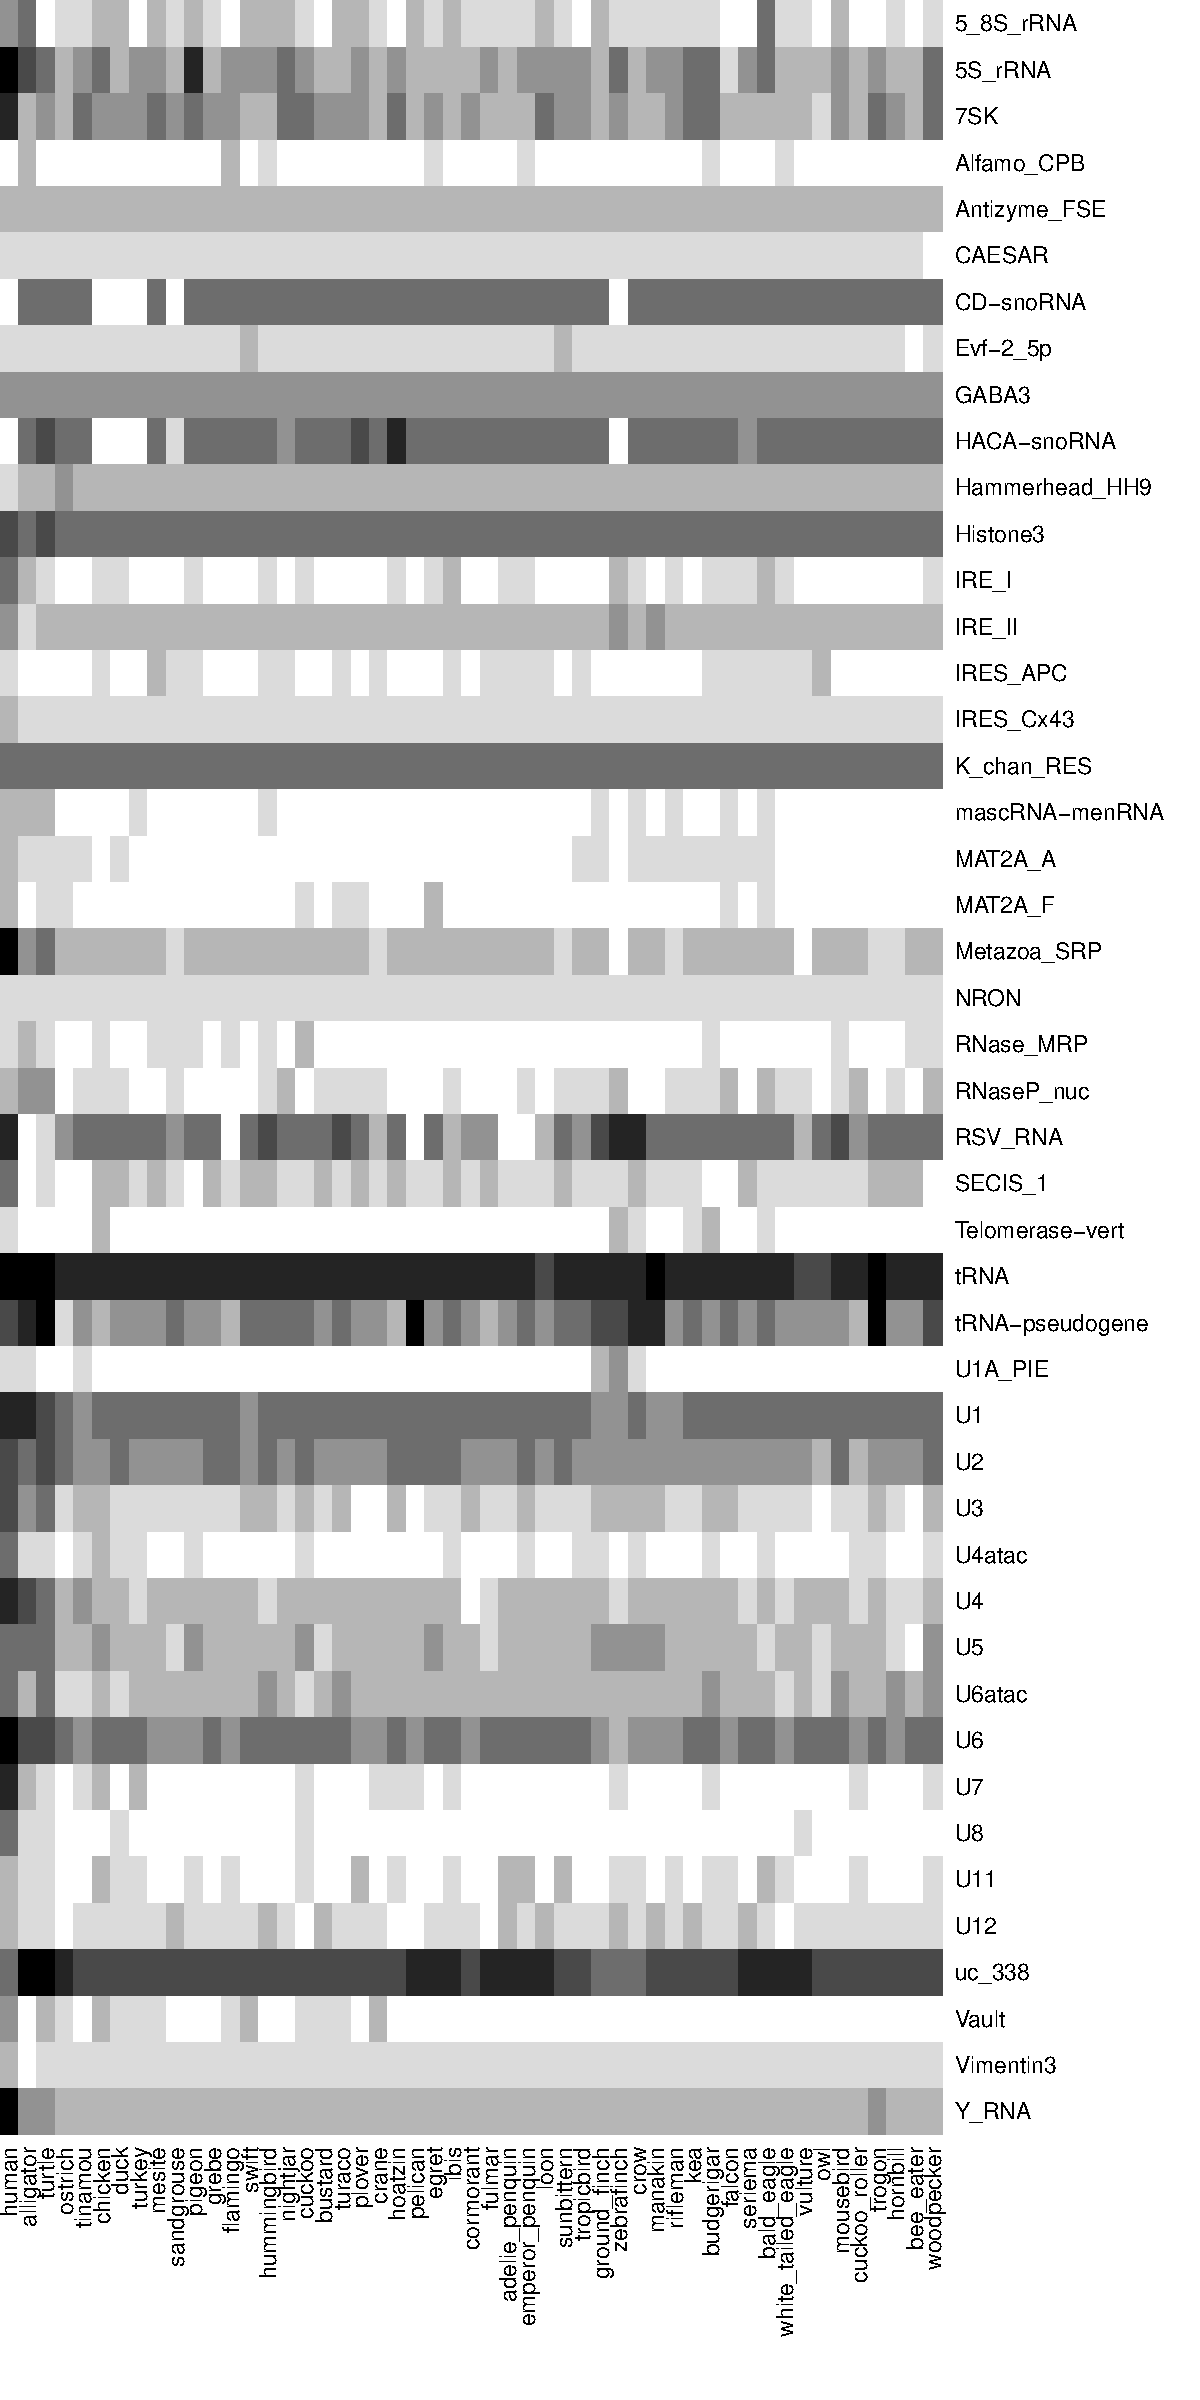
\includegraphics[width=0.4\textwidth]{figures/RNA.pdf}
  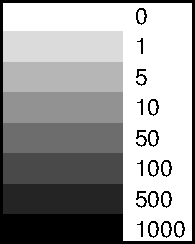
\includegraphics[width=0.1\textwidth]{figures/key2.pdf}
  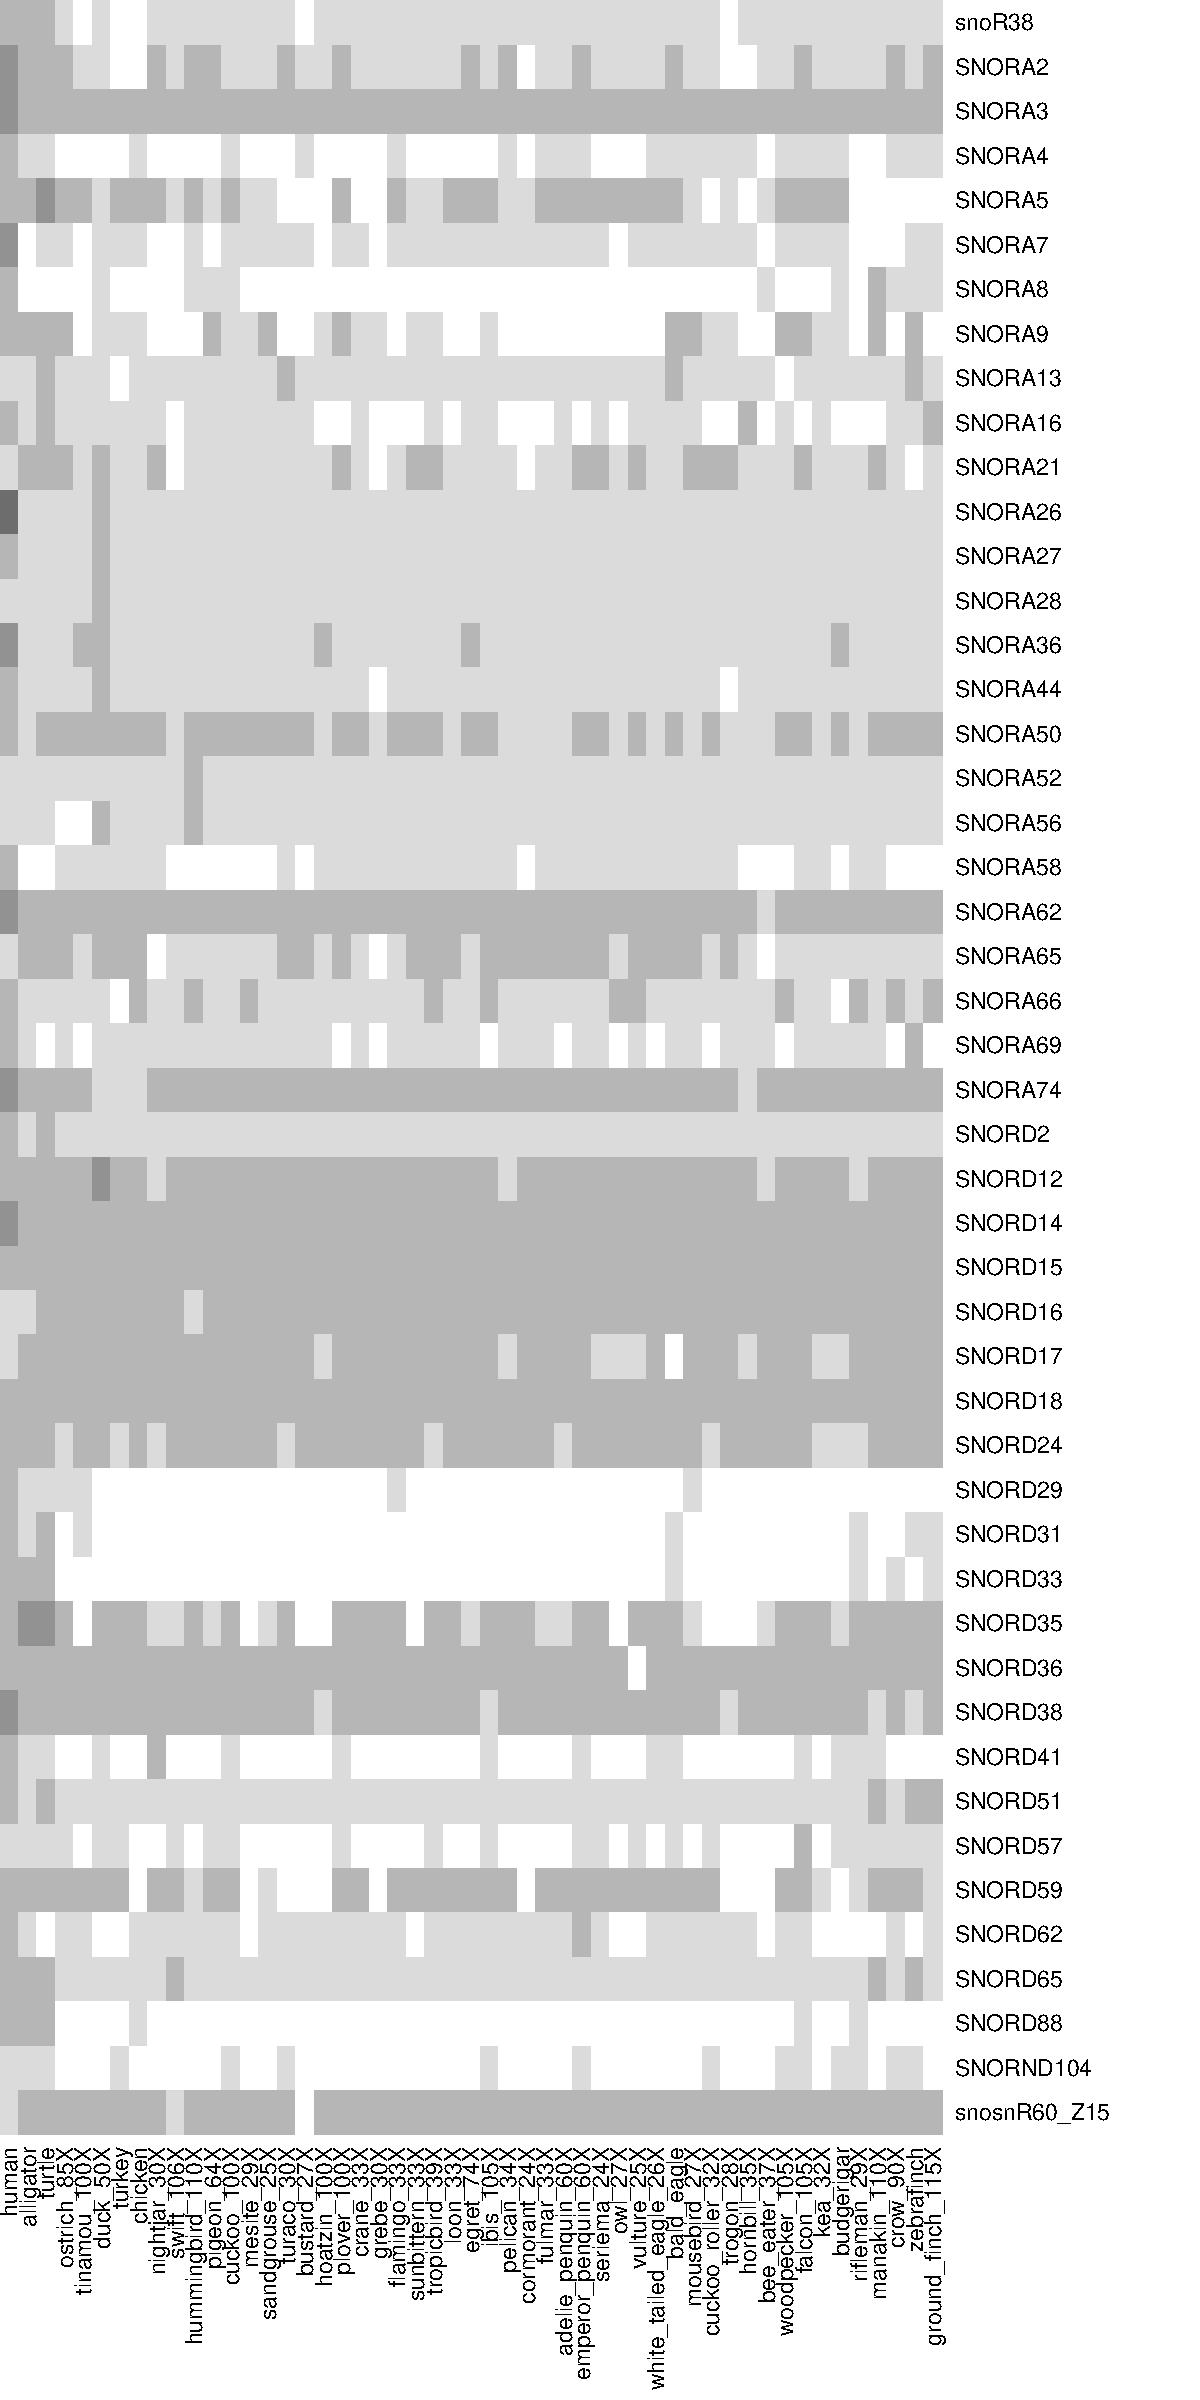
\includegraphics[width=0.4\textwidth]{figures/snoRNA-human-yeast-correspondences.pdf}
  \caption[]{This figure illustrates the number of copies of Rfam and
    tRNAscan annotations for each RNA family in each avian species and
    outgroups. The families are ordered alphabetically vertically and
    the species are in phylogenetic order horizontally. Darker shades
    indicate high copy numbers, lighter shades indicate fewer, white
    indicates no predictions were made.}\label{fig:1}
\end{figure}

\begin{figure}[ht]
  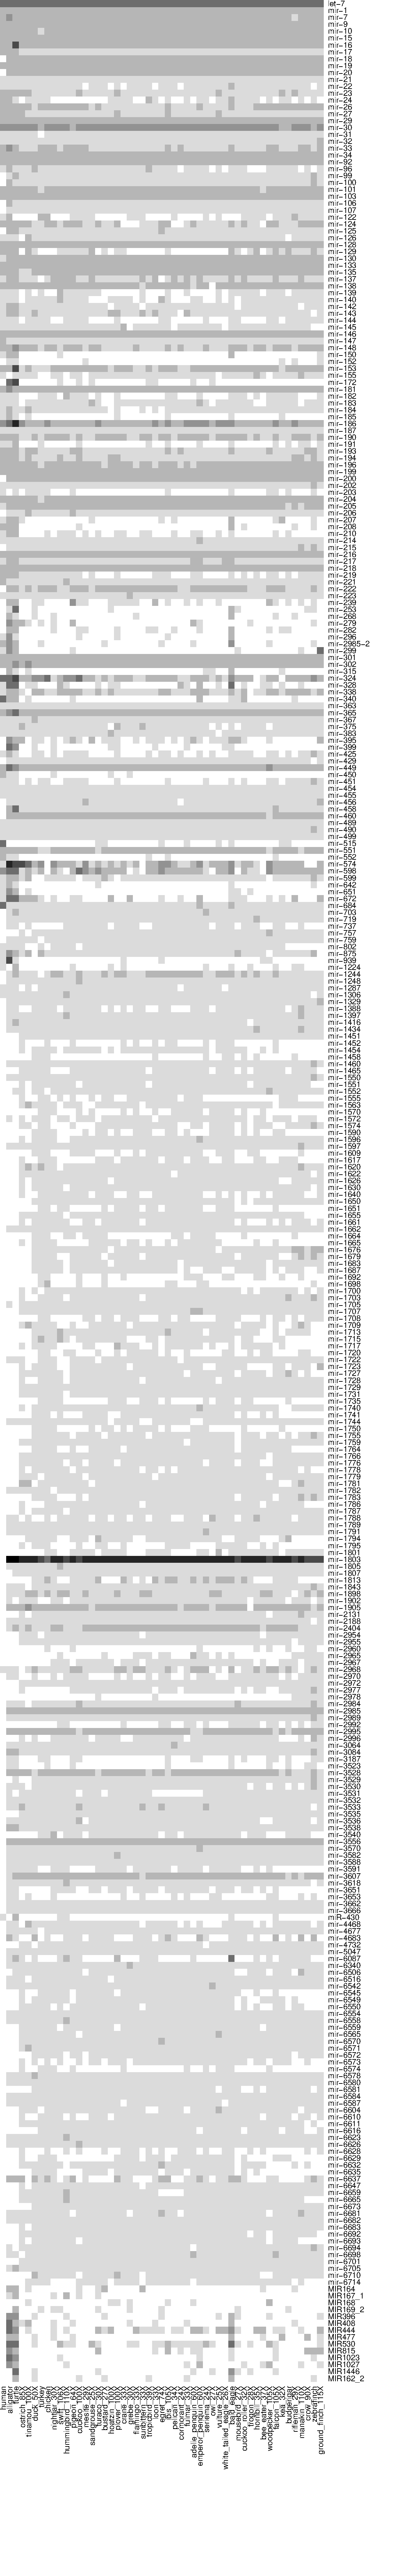
\includegraphics[height=0.95\textheight]{figures/miRNA.pdf}
  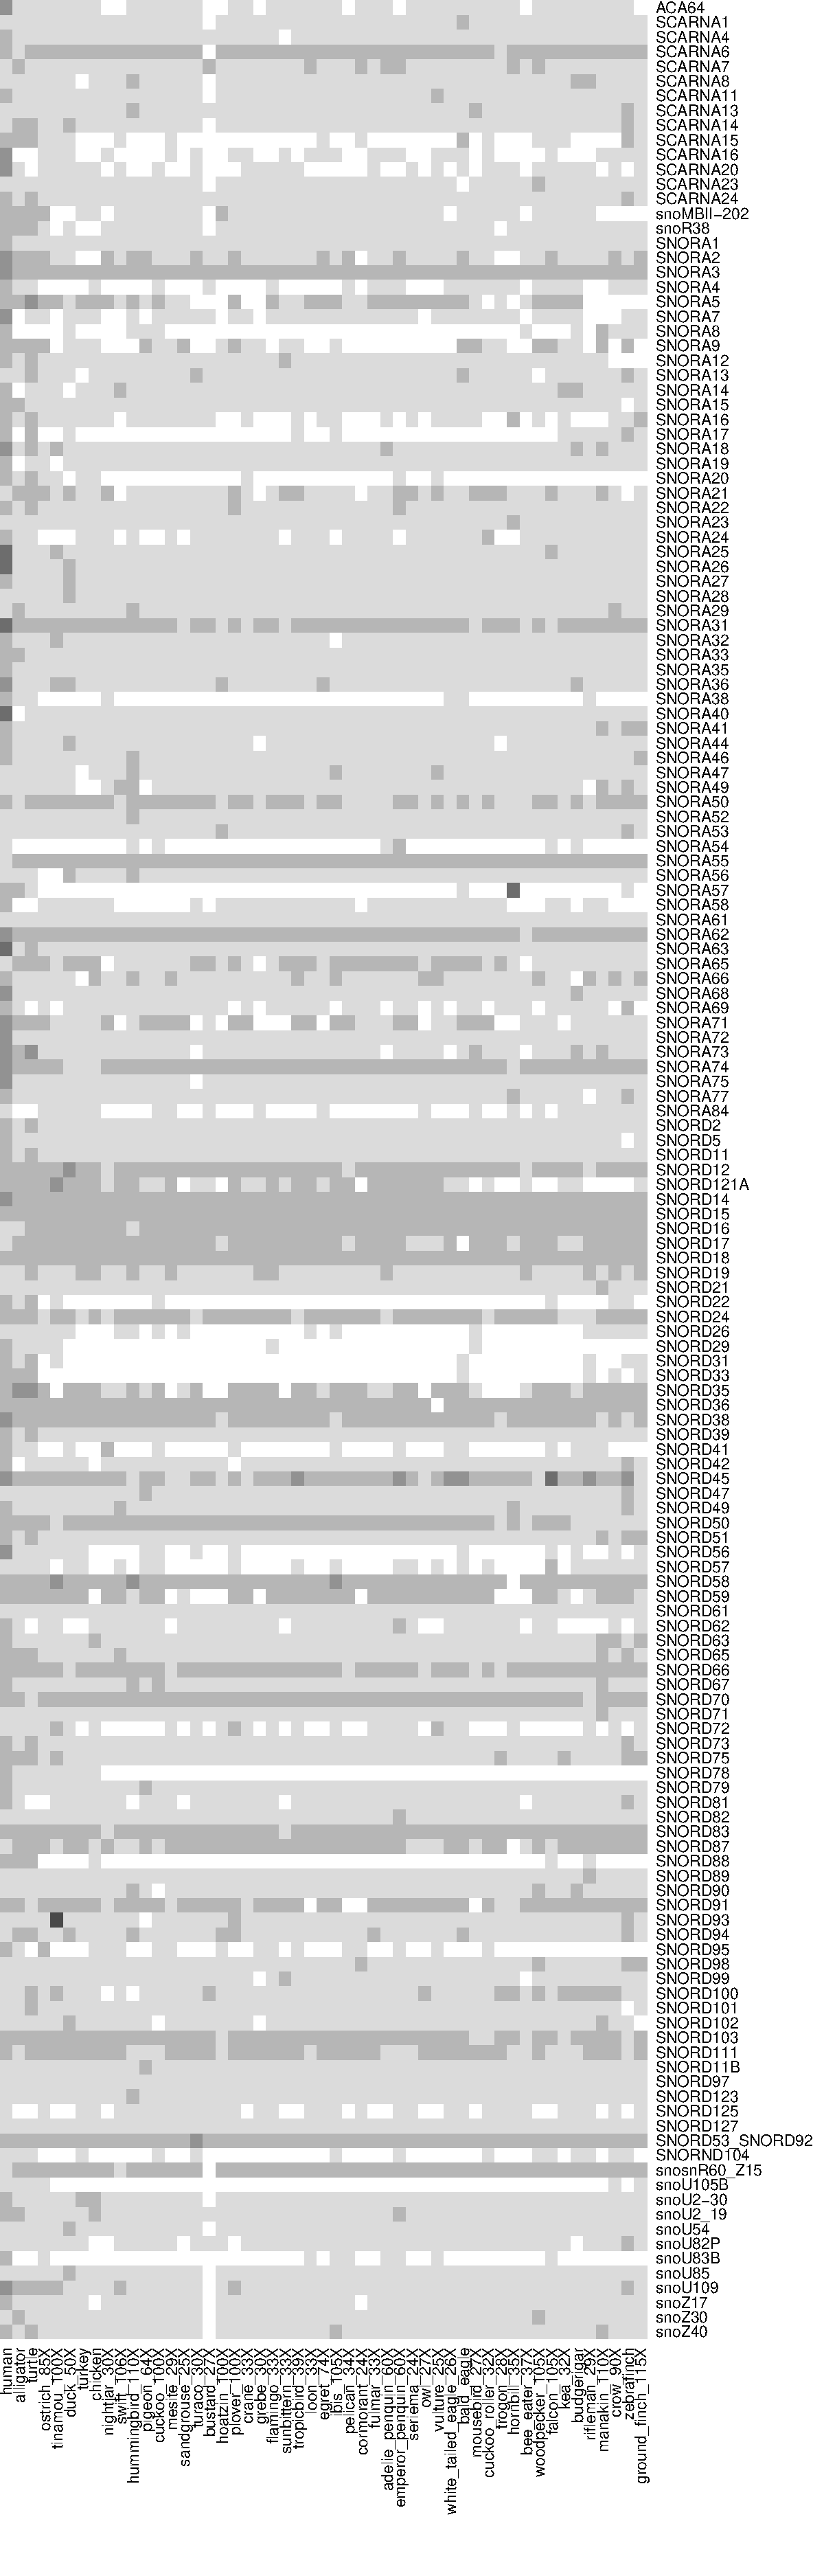
\includegraphics[height=0.95\textheight]{figures/snoRNA.pdf}
  \caption[]{Heatmaps showing the prescence/abscence and approximate
    copy number of {\bf miRNA} families on the right and {\bf snoRNA} families on
    the left.}\label{fig:3}
\end{figure}

\begin{figure}[ht]
  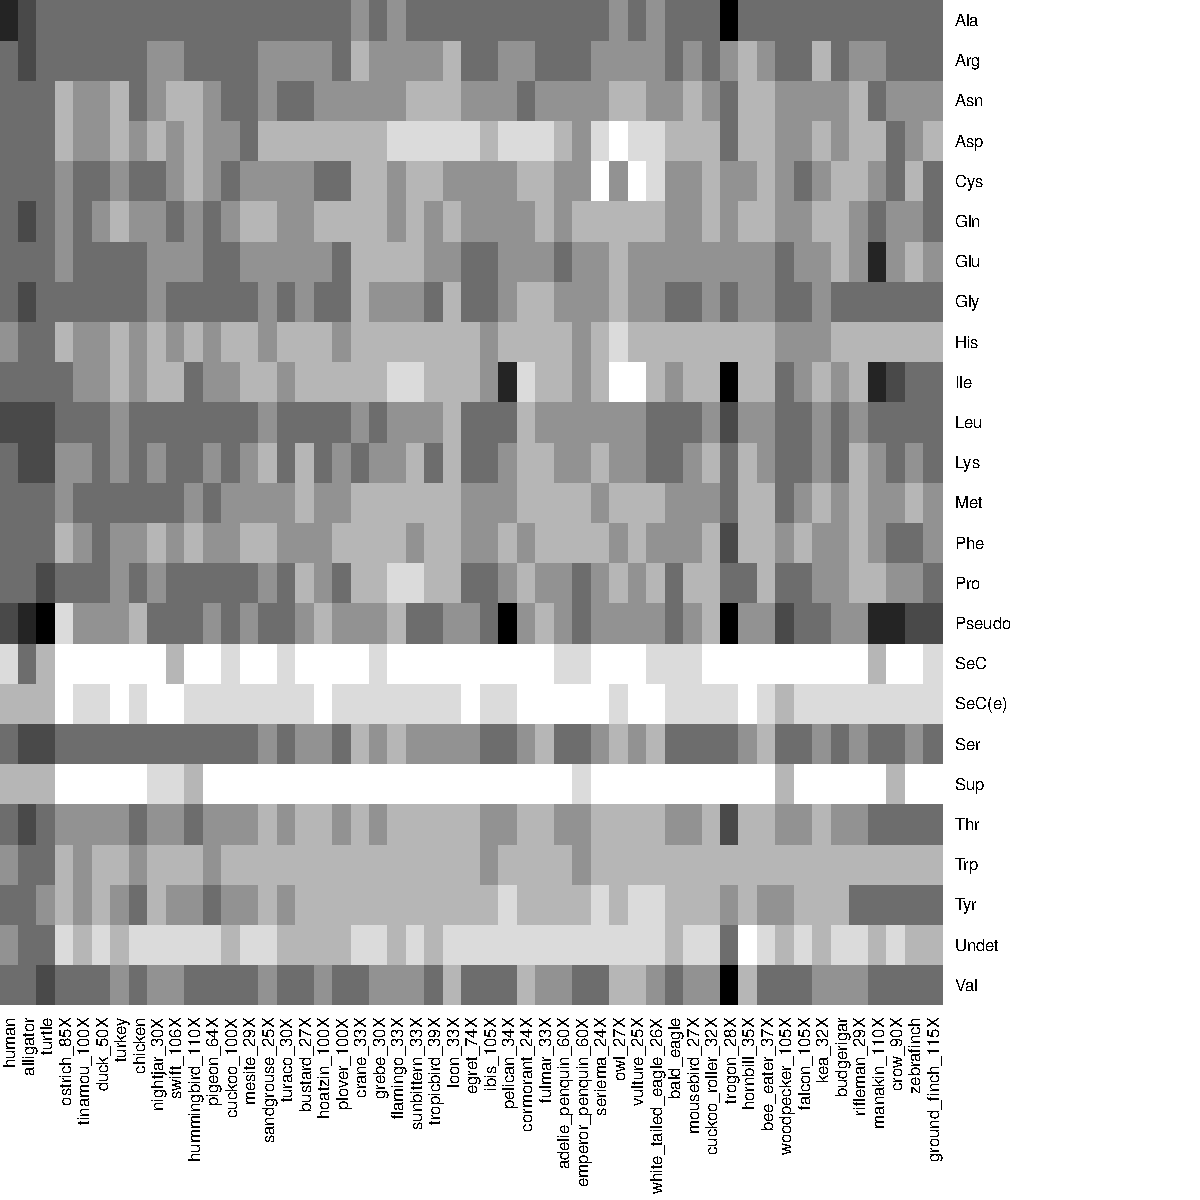
\includegraphics[width=0.85\textwidth]{figures/tRNA.pdf}
  \caption[]{Heatmaps showing the prescence/abscence and approximate
    copy number of {\bf tRNA} families.}\label{fig:5}
\end{figure}

\begin{figure}[ht]
  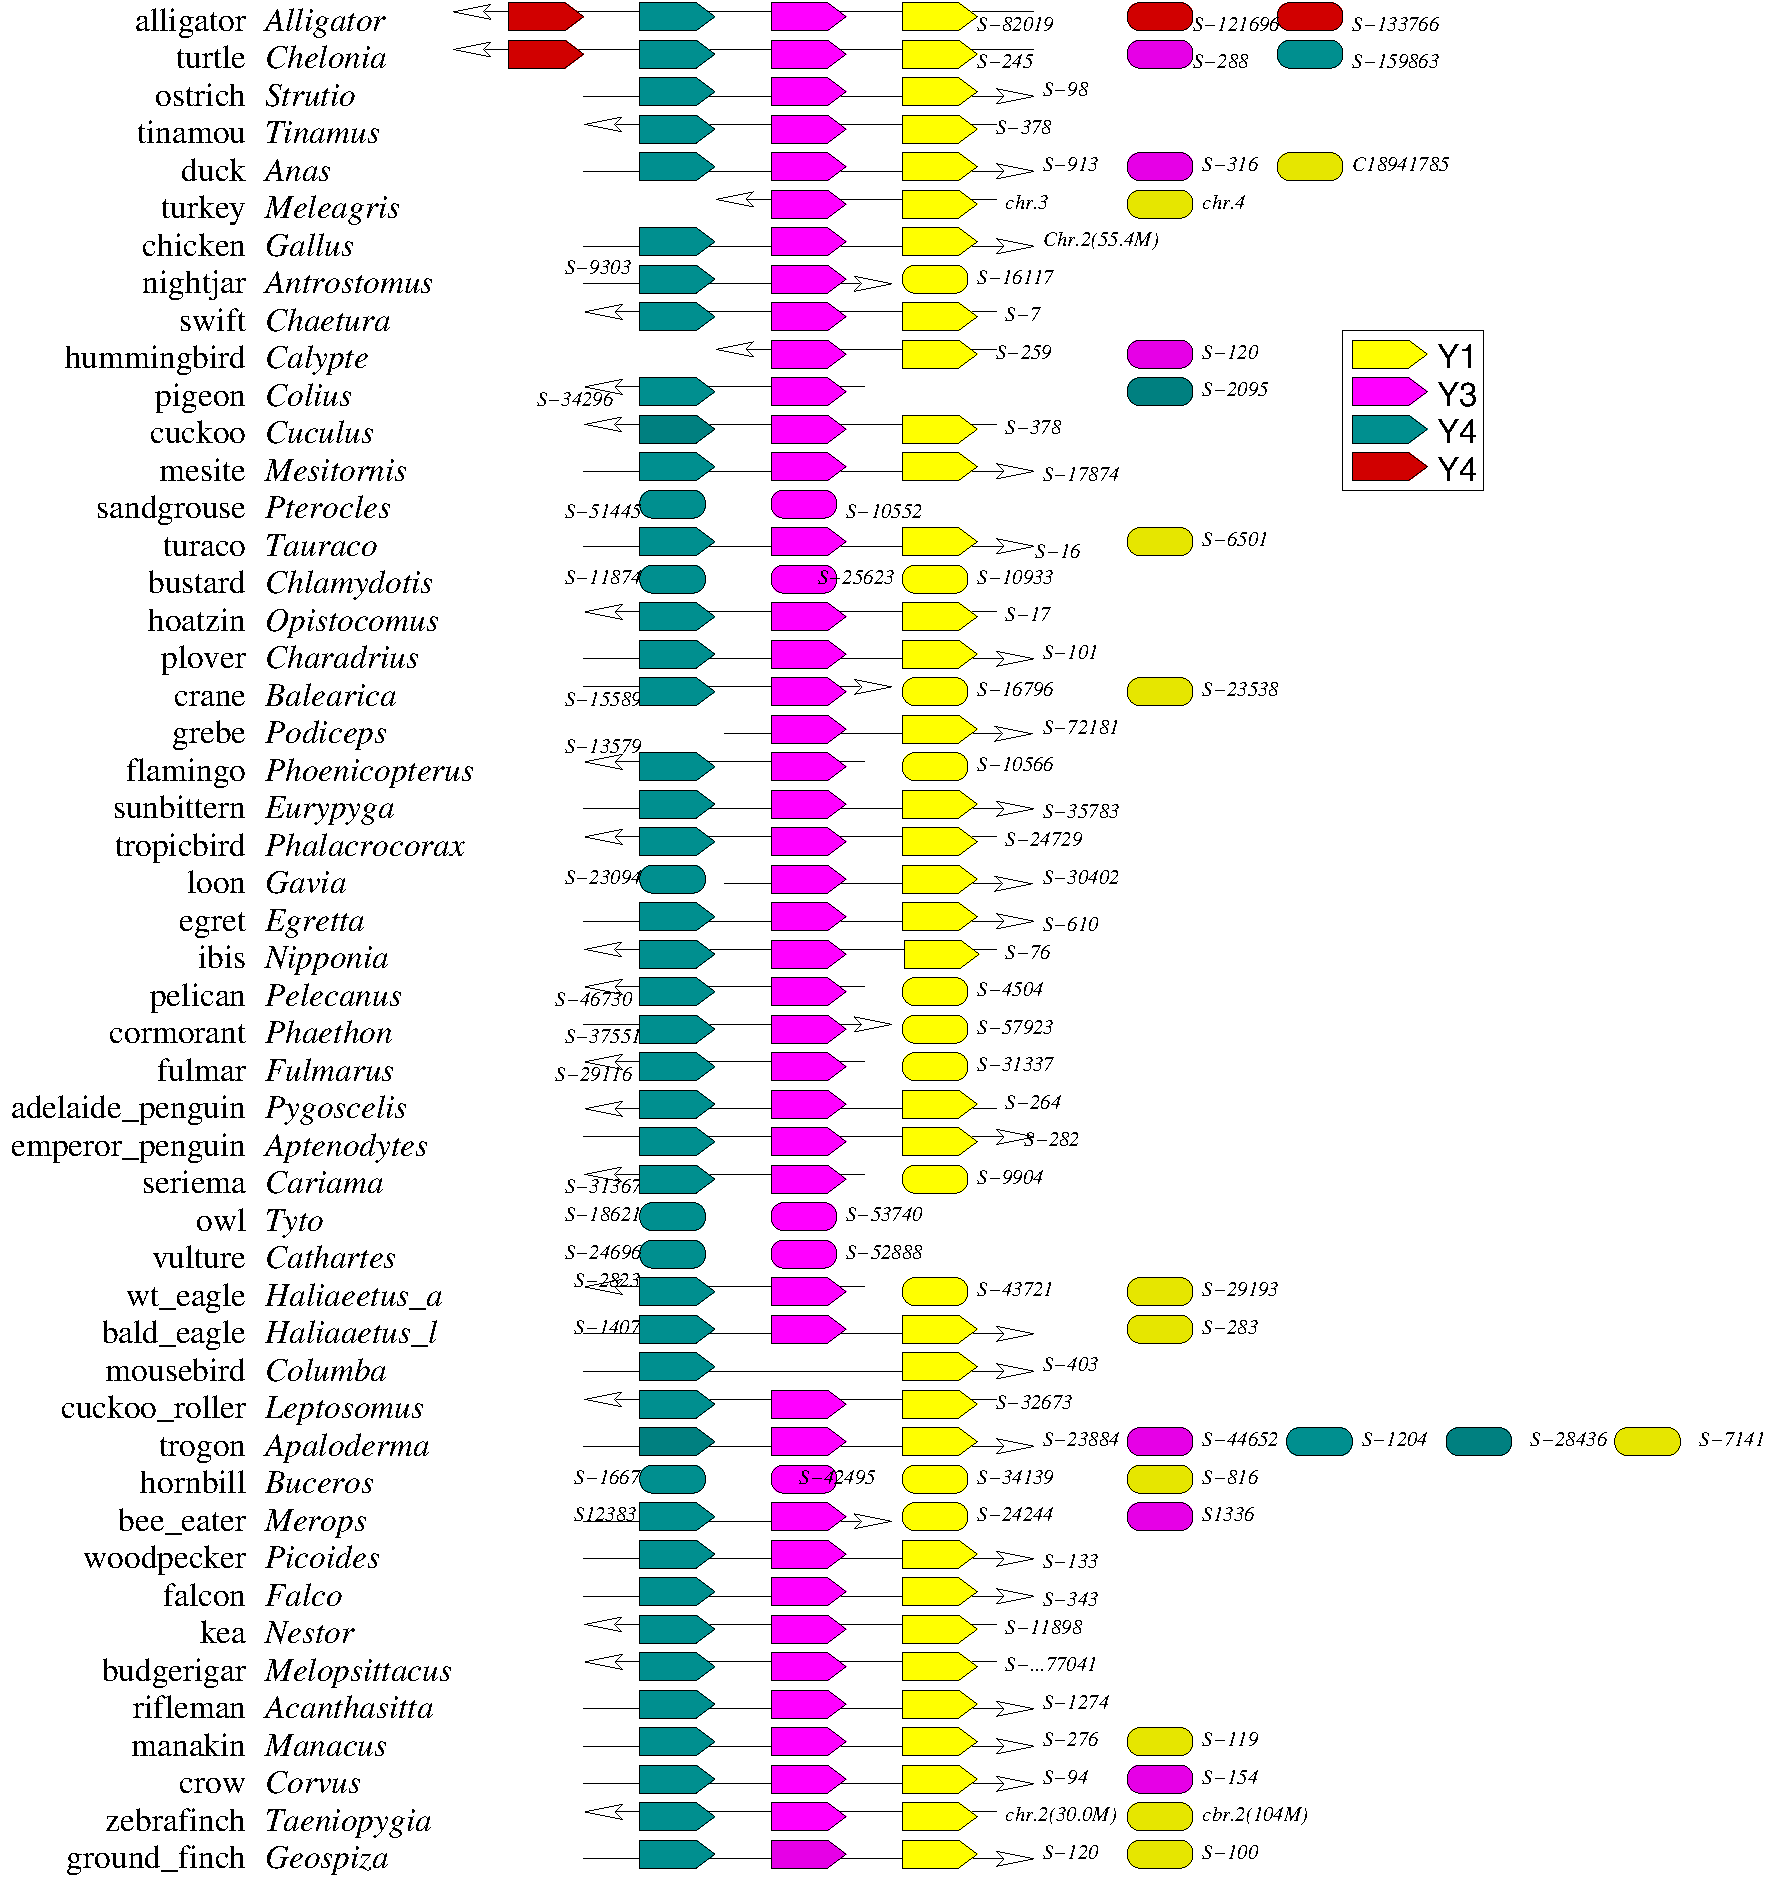
\includegraphics[width=0.95\textwidth]{figures/Y.pdf}
  \caption[]{Syntenic conservation of the Y RNA cluster in avian and
    reptile genomes.}\label{fig:6}
\end{figure}

\begin{figure}[ht]
  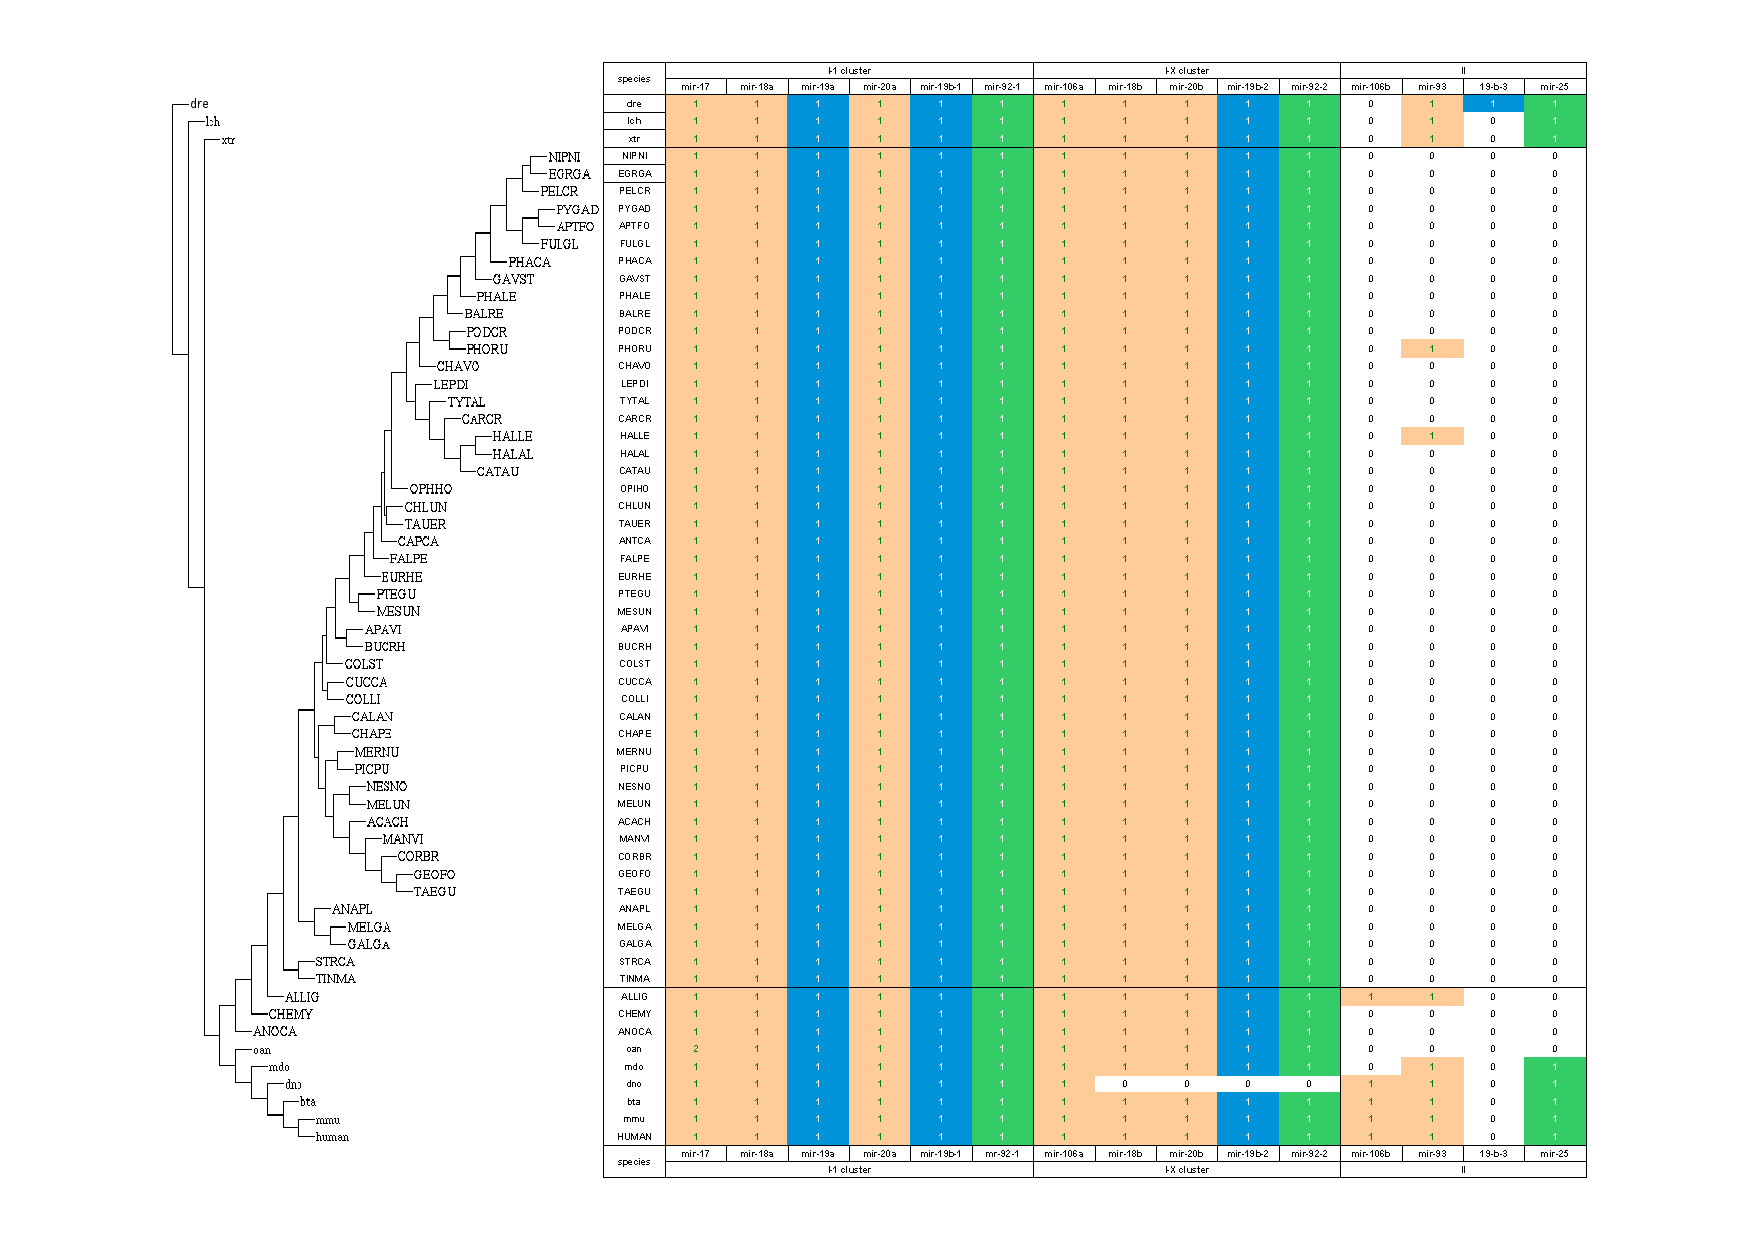
\includegraphics[width=0.95\textwidth]{figures/mir-17-cluster.pdf}
  \caption[Presence/absence table of mir-17 miRNA clusters]{ This
    figure illustrates the distribution of all members of the mir-17
    clusters across birds, compared to fish and mammals. Columns
    correspond to single miRNA sequences, grouped by clusters and
    ordered by their position within the corresponding cluster. Rows
    correspond to the species and the cells contain the number of
    copies of the miRNA in the respective species. Colors correspond
    to orthologous miRNA families: mir-17 (orange), mir-19 (blue) and
    mir-92/25 (green).There are 3 clusters, I-1 and I-X, and cluster
    II.  While the two copies of cluster I are completely conserved,
    cluster II has been lost as a whole in birds.}\label{fig:8}
\end{figure}



\begin{figure}[ht]
  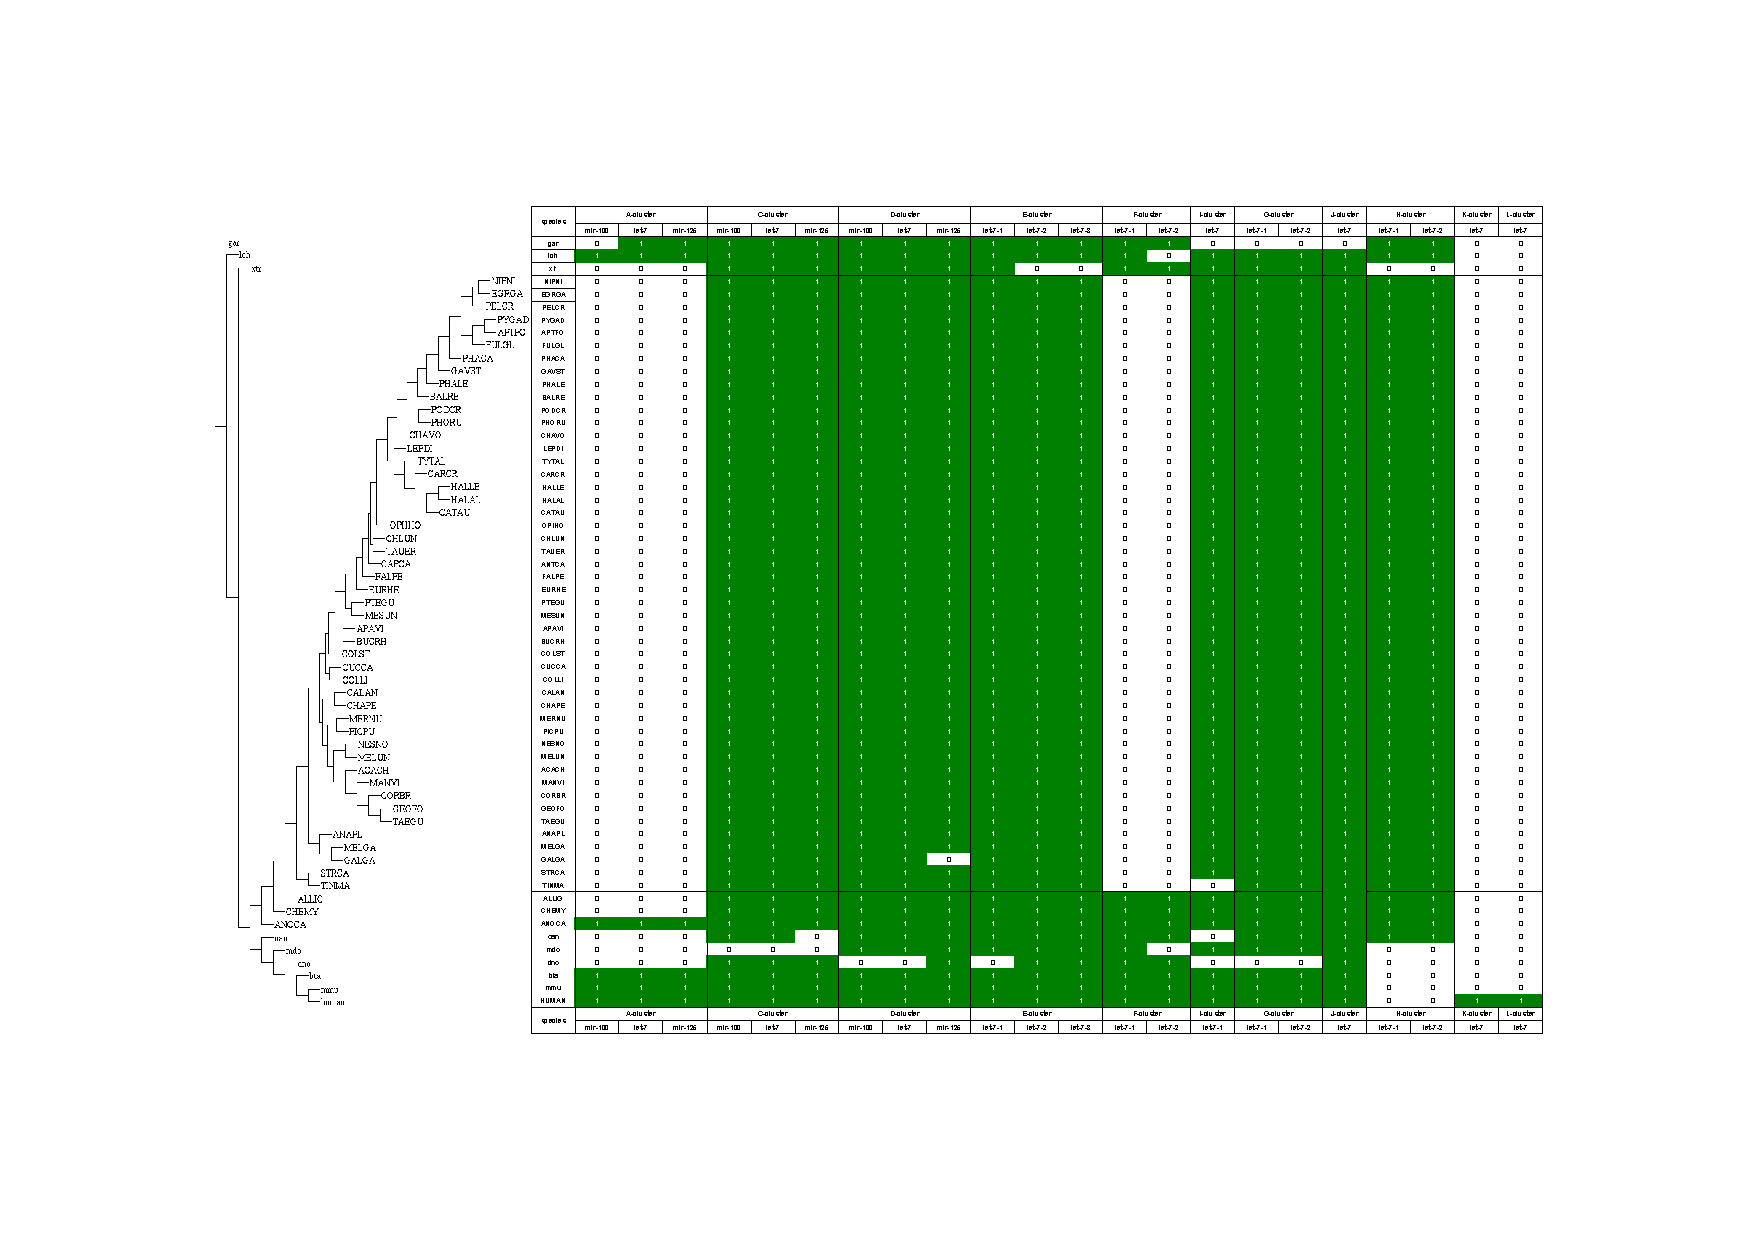
\includegraphics[width=0.95\textwidth]{figures/let-7-cluster.pdf}
  \caption[Presence/absence table of let-7 miRNA clusters]{This figure
    illustrates the distribution of the let-7 paralogs and clustered
    miRNAs of the families mir-100 and mir-125. Columns correspond to
    single miRNA sequences, grouped by clusters and ordered by their
    position within the corresponding cluster. Rows correspond to the
    species and the cells contain the number of copies of the miRNA in
    the respective species. Cluster A, which is strongly conserved in
    vertebrates has been completely lost in the avian lineage. Another
    obvious loss in birds is cluster F. However, in tinamou we
    detected an unclustered miRNA that best fits to F-let-7-1 in
    sequence and structure, while we could not find an I-let-7 miRNA
    sequence in this species.}\label{fig:9}
\end{figure}



\begin{figure}[ht]
%\includegraphics[width=0.99\textwidth]{/home/ppg15/people/birds/mario/chr1-147253243-147253923-miRNA-cluster.pdf}
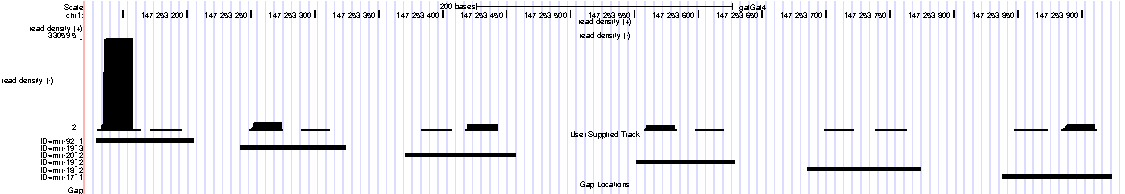
\includegraphics[width=0.99\textwidth]{figures/mir-17-I-1-cluster.pdf}
  \caption[]{microRNA 17 I-1 cluster: mir-92\_1, mir-19\_3, mir-20\_2,
    mir-19\_2, mir-18\_2 \& mir-17\_1. The figure indicates the
    genomic location and the RNA-seq read-depths for these 6
    microRNAs.}\label{fig:10}
\end{figure}

\begin{figure}[ht]
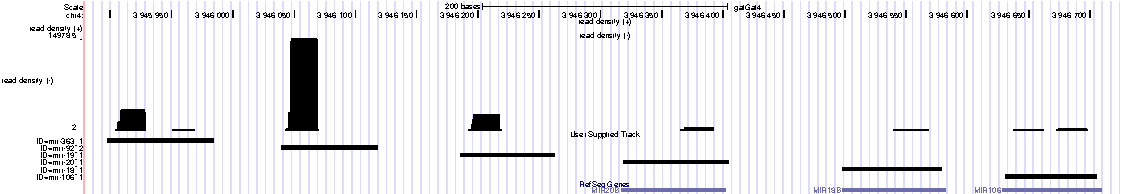
\includegraphics[width=0.99\textwidth]{figures/mir-17-I-X-cluster.pdf}
  \caption[]{microRNA 17 I-X cluster: mir-363\_1, mir-92\_2,
    mir-19\_1, mir-20\_1, mir-18\_1, mir-106\_1. The figure indicates
    the genomic location and the RNA-seq read-depths for these 6
    microRNAs.}\label{fig:11}
\end{figure}

\begin{figure}[ht]
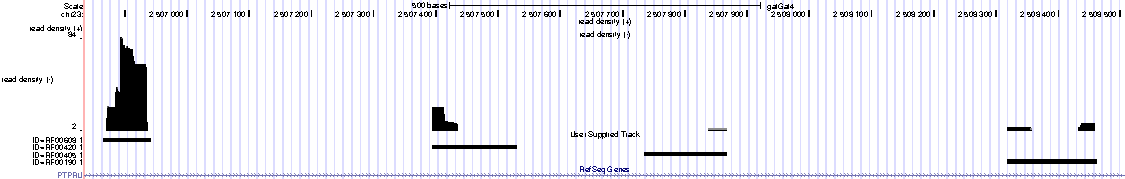
\includegraphics[width=0.99\textwidth]{figures/chr23-2507395-2508461-snoRNA-cluster.pdf}
  \caption[]{H/ACA box snoRNA cluster: SNORA61, SNORA44, SNORA16. The figure indicates
    the genomic location and the RNA-seq read-depths for these 3
    snoRNAs.}\label{fig:12}
\end{figure}

\begin{figure}[ht]
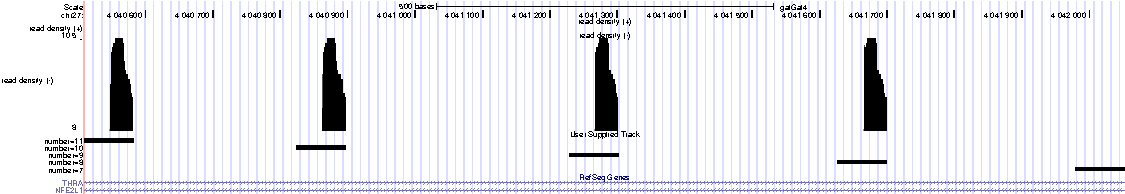
\includegraphics[width=0.99\textwidth]{figures/chr27-4040511-4042052-tRNA-cluster.pdf}
  \caption[]{Cysteine tRNA cluster. The figure indicates
    the genomic location and the RNA-seq read-depths for these 5
    transfer RNAs.}\label{fig:13}
\end{figure}

\begin{figure}[ht]
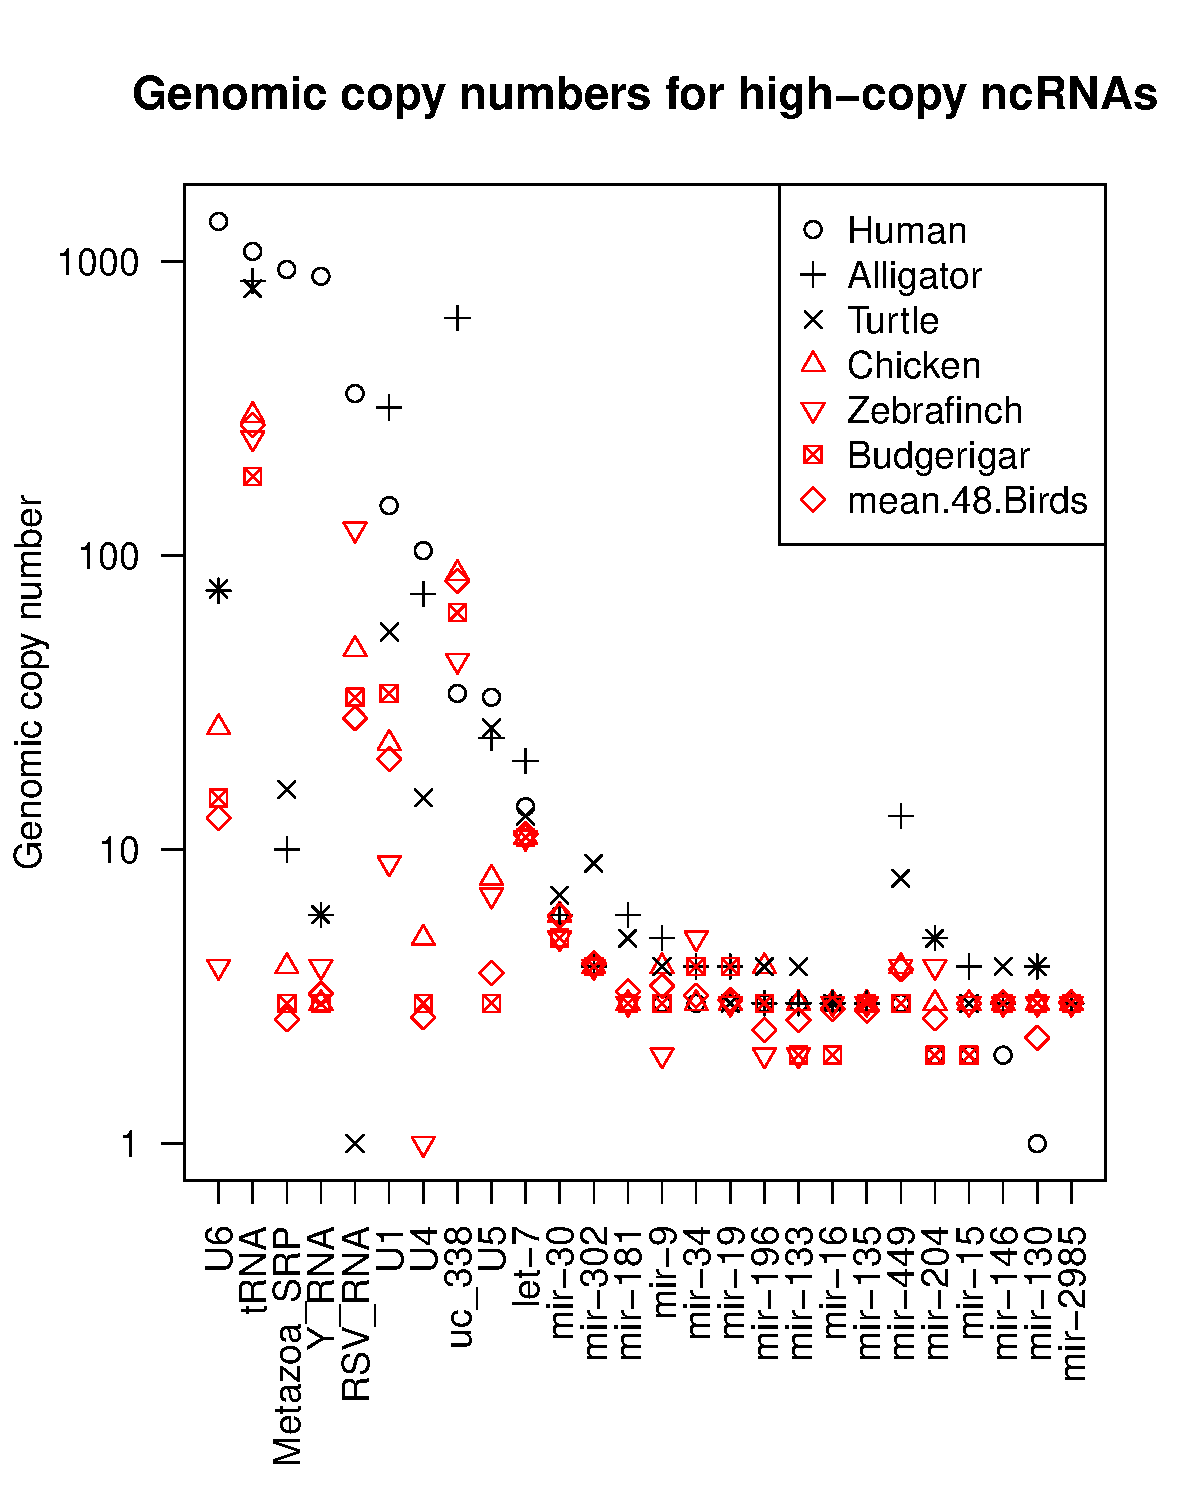
\includegraphics[width=0.475\textwidth]{figures/high-copy-numbers.pdf}
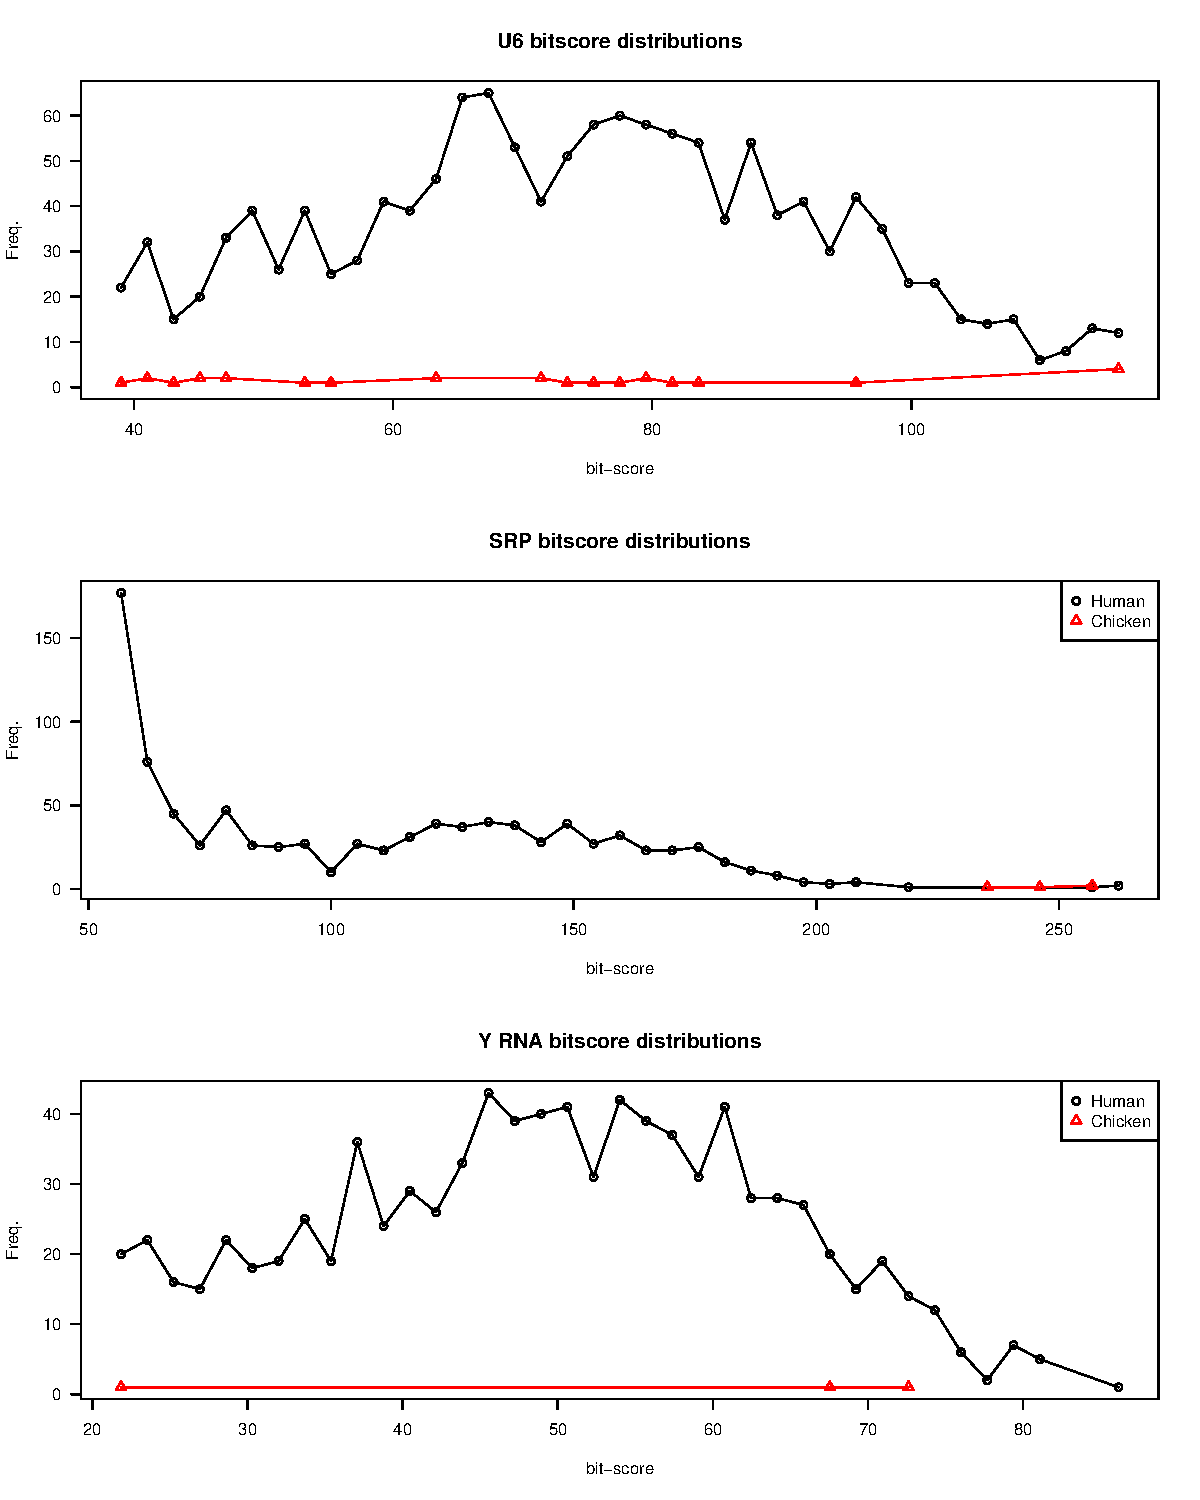
\includegraphics[width=0.475\textwidth]{figures/high-copy-numbers-U6-SRP.pdf}
  \caption[]{{\bf Left:} A comparison of the genomic copy numbers for
    26 of the most abundant RNAs found in human, reptile and the bird
    genomes. {\bf Right:} Bit-score distributions for the Rfam U6,
    Metazoan SRP and the Y RNA covariance models for human and chicken
    paralogues/pseudogenes. Loci with high bit-scores are more likely
    to be functional than those with low bit-scores (due to excess
    variation that conflicts with the canonical RNA
    models).}\label{fig:14}
\end{figure}

\clearpage
\newpage

\begin{figure}[ht]
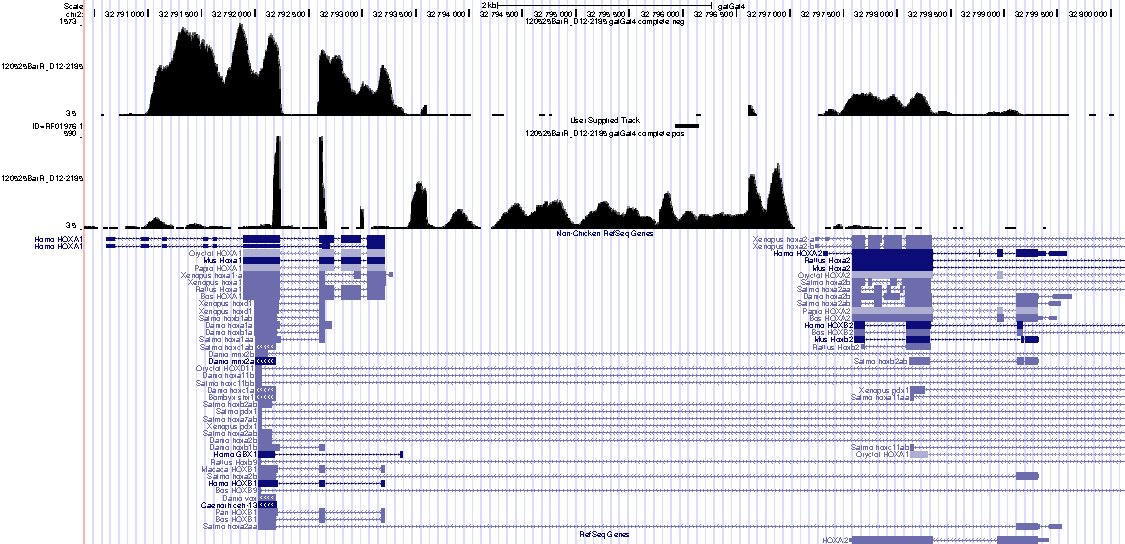
\includegraphics[width=0.99\textwidth]{figures/HOTAIR_loci_expression.pdf}
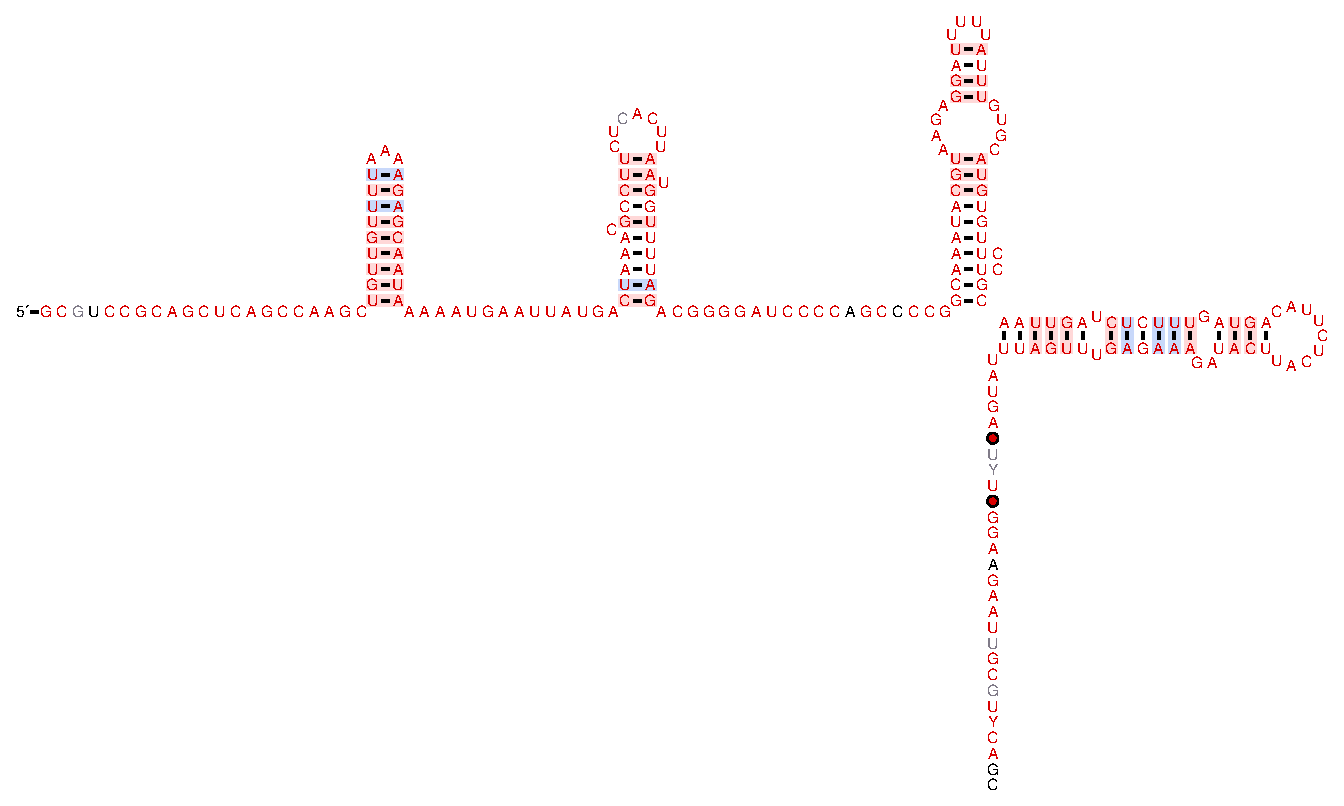
\includegraphics[width=0.99\textwidth]{figures/HOTAIRM1_2.pdf}
  \caption[]{Above: Expression of the chicken HOTAIRM1 (RF01976) locus
    and the surrounding genes: HOXA1, HOXA2, and HOXA3. Below: The
    predicted secondary structure of the Avian HOTAIRM1 domain.}\label{fig:15}
\end{figure}

\begin{figure}[ht]
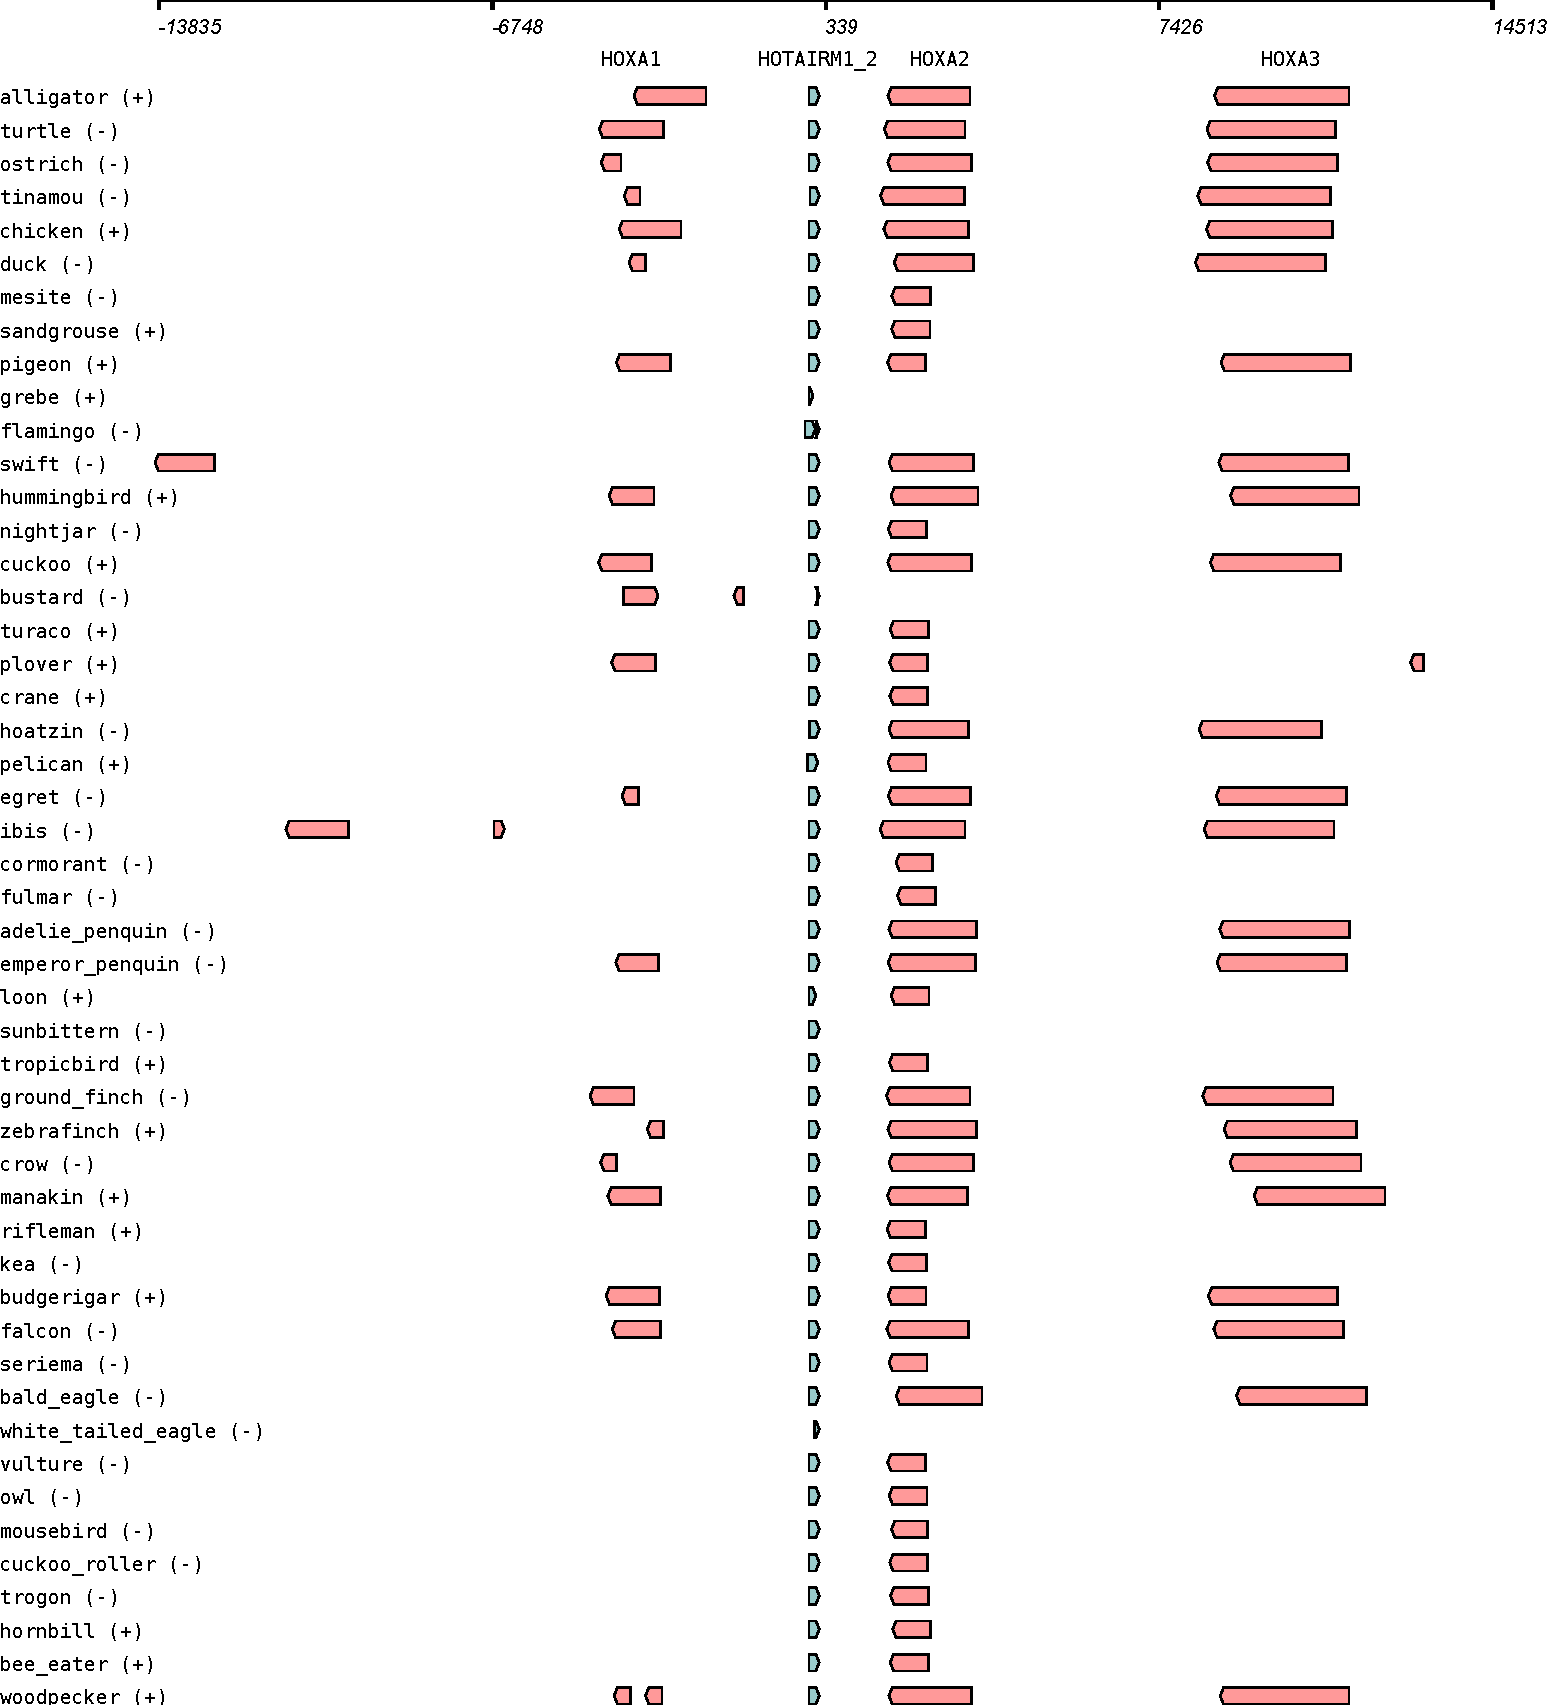
\includegraphics[width=0.99\textwidth]{figures/HOTAIR_loci_synteny.pdf}
  \caption[]{The preservation of gene order (synteny) surrounding the
    HOTAIRM1 (RF01976) locus across the Avian and other Vertebrate
    lineages.}\label{fig:16}
\end{figure}

\clearpage
\newpage

\begin{table}[h!]
  \begin{center}
    \begin{tabular}{|l|l|r|c|}
    \hline
RNA family (Rfam ID) & Chromosome & Coordinates & Strand \\
    \hline
\multicolumn{4}{|l|}{Macro-chromosomes:}\\
RNase MRP (RF00030)     & chr4 & 39276202-39276488 & -\\
\multicolumn{4}{|l|}{Micro-chromosomes:}\\ 
U4atac snRNA (RF00618)  & chr7 &	25702714-25702831 & +\\
RNase P RNA (RF00009)   & chr8 & 6609347-6609668   & -\\
Telomerase RNA (RF00024)& chr9 & 19429028-19429084 & +\\
Vault RNA (RF00006)     & chr13& 380747-380840     & +\\
U11 snRNA (RF00548)     & chr23& 2216932-2217058   & -\\
\hline
    \end{tabular}
  \end{center}
  \caption{The location of ``missing'' RNA families in the chicken genome (galGal4). }
\end{table}


\clearpage
\newpage

\begin{figure}[ht]
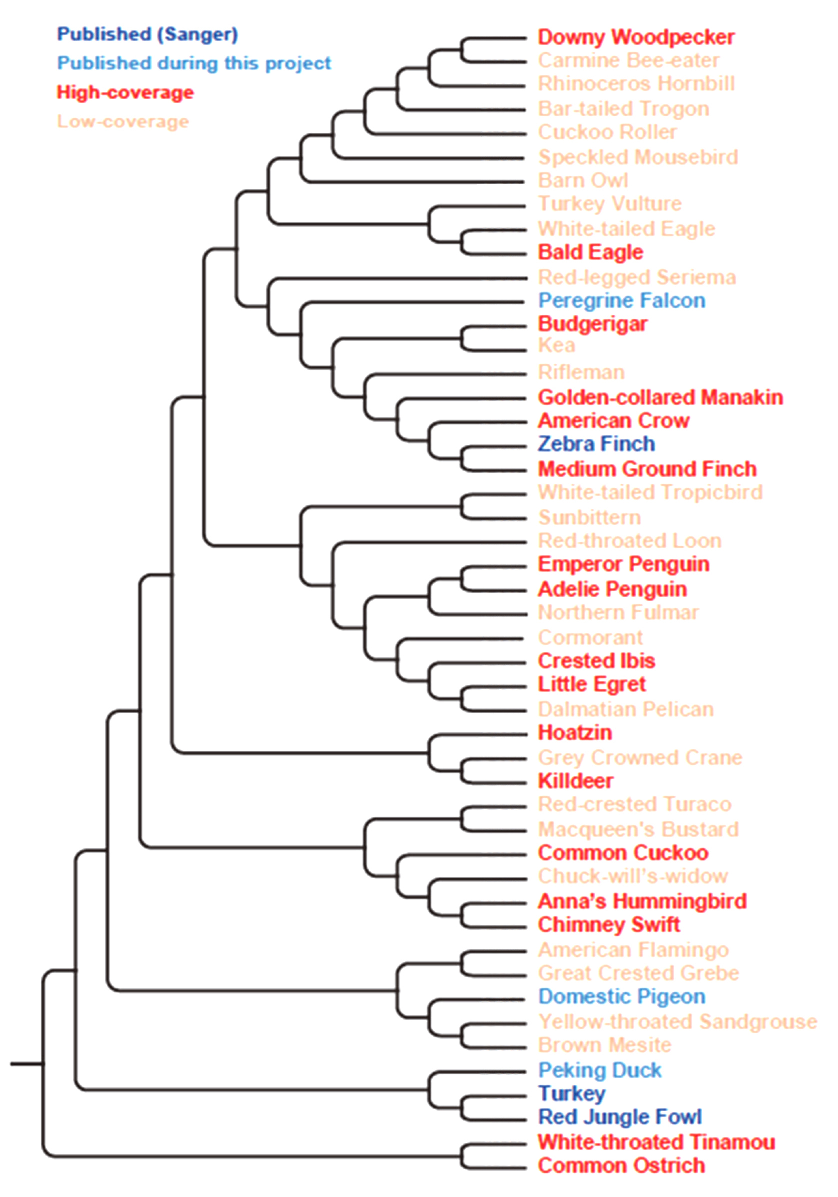
\includegraphics[width=0.9\textwidth]{figures/phylo-tree.pdf}
  \caption[]{The phylogenetic relationships between the Avian species
    used in this study. This figure has been reproduced, with permission from \cite{birds:14a}.}\label{fig:17}
\end{figure}



\clearpage
\newpage


\subsection*{Database accessions}

The NCBI BioProject, SRA and Study IDs for the genomes used in this study
are are listed below.

\begin{table}[h!]
  \begin{center}
    \begin{tabular}{|l|l|l|l|}
    \hline
Species & BioProject ID & SRA ID & Study ID \\
    \hline
\emph{Chaetura pelagica} & PRJNA210808  & SRA092327 & SRP026688\\
\emph{Calypte anna} & PRJNA212866 & SRA096094 & SRP028275\\
\emph{Charadrius vociferus} & PRJNA212867 & SRA096158 & SRP028286\\
\emph{Corvus brachyrhynchos} & PRJNA212869 & SRA096200 & SRP028317\\
\emph{Cuculus canorus} & PRJNA212870 & SRA096365 & SRP028349\\
\emph{Manacus vitellinus} & PRJNA212872 & SRA096507 & SRP028393\\
\emph{Ophisthocomus hoazin} & PRJNA212873 & SRA096539 & SRP028409\\
\emph{Picoides pubescens} & PRJNA212874 & SRA097131 & SRP028625\\
\emph{Struthio camelus} & PRJNA212875 & SRA097407 & SRP028745\\
\emph{Tinamus guttatus} & PRJNA212876 & SRA097796 & SRP028753\\
\emph{Acanthisitta chloris} & PRJNA212877 & SRA097960 & SRP028832\\
\emph{Apaloderma vittatum} & PRJNA212878 & SRA097967 & SRP028834\\
\emph{Balearica regulorum} & PRJNA212879 & SRA097970 & SRP028839\\
\emph{Buceros rhinoceros} & PRJNA212887 & SRA097991 & SRP028845\\
\emph{Antrostomus carolinensis} & PRJNA212888 & SRA098079 & SRP028883\\
\emph{Cariama cristata} & PRJNA212889 & SRA098089 & SRP028884\\
\emph{Cathartes aura} & PRJNA212890 & SRA098145 & SRP028913\\
\emph{Chlamydotis macqueenii} & PRJNA212891 & SRA098203 & SRP028950\\
\emph{Colius striatus} & PRJNA212892 & SRA098342 & SRP028965\\
\emph{Eurypyga helias} & PRJNA212893 & SRA098749 & SRP029147\\
\emph{Fulmarus glacialis} & PRJNA212894 & SRA098806 & SRP029180\\
\emph{Gavia stellata} & PRJNA212895 & SRA098829 & SRP029187\\
\emph{Haliaeetus albicilla} & PRJNA212896 & SRA098868 & SRP029203\\
\emph{Haliaeetus leucocephalus} & PRJNA237821 & SRX475899 & SRP038924\\
                         & SRX475900   &           &          \\
                         & SRX475901   &           &          \\
                         & SRX475902   &           &          \\
\emph{Leptosomus discolor} & PRJNA212897 & SRA098894 & SRP029206\\
\emph{Merops nubicus} & PRJNA212898 & SRA099305 & SRP029278\\
\emph{Mesitornis unicolor} & PRJNA212899 & SRA099409 & SRP029309\\
\emph{Nestor notabilis} & PRJNA212900 & SRA099410 & SRP029311\\
\emph{Pelecanus crispus} & PRJNA212901 & SRA099411 & SRP029331\\
\emph{Phaethon lepturus} & PRJNA212902 & SRA099412 & SRP029342\\
\emph{Phalacrocorax carbo} & PRJNA212903 & SRA099413 & SRP029344\\
\emph{Phoenicopterus ruber} & PRJNA212904 & SRA099414 & SRP029345\\
\emph{Podiceps cristatus} & PRJNA212905 & SRA099415 & SRP029346\\
\emph{Pterocles gutturalis} & PRJNA212906 & SRA099416 & SRP029347\\
\emph{Tauraco erythrolophus} & PRJNA212908 & SRA099418 & SRP029348\\
\emph{Tyto alba} & PRJNA212909 & SRA099419 & SRP029349\\
\emph{Nipponia nippon} & PRJNA232572 & SRA122361 & SRP035852\\
\emph{Egretta garzetta} & PRJNA232959 & SRA123137 & SRP035853\\
\hline
    \end{tabular}
  \end{center}
  \caption{The NCBI BioProject/SRA and Study IDs used in this study. }
\end{table}



\begin{table}[h!]
  \begin{center}
    \begin{tabular}{|l|l|l|l|}
    \hline
Species & BioProject ID & SRA ID & Study ID \\
    \hline
\multicolumn{4}{|l|}{Genomes released before}\\
\hline
\emph{Aptenodytes forsteri} & PRJNA235982 & SRA129317 & SRP035855\\
\emph{Pygoscelis adeliae} & PRJNA235983 & SRA129318 & SRP035856\\
\emph{Gallus gallus} & PRJNA13342 & SRA030184 & SRP005856 (galGal4)\\
\emph{Taeniopygia guttata} & PRJNA17289 & SRA010067 & SRP001389\\
\emph{Meleagris gallopavo} & PRJNA42129 & Unknown & Unknown\\
\emph{Melopsittacus undulatus} & PRJEB1588 & ERA200248 & ERP002324\\
\emph{Anas platyrhynchos} & PRJNA46621 & SRA010308 & SRP001571\\
\emph{Columba livia} & PRJNA167554 & SRA054954 & SRP013894\\
\emph{Falco peregrinus} & PRJNA159791 & SRA055082 & SRP013939\\
\emph{Geospiza fortis} & PRJNA156703 & SRA051234 & SRP011940\\
\hline
\multicolumn{4}{|l|}{Outgroups}\\
\hline
\emph{Homo sapiens} & & & HG19/GRCh37\\
\emph{Alligator mississippiensis} & & & allMis1\\
\emph{Chelonia mydas} & PRJNA104937 & & \\
\hline
\multicolumn{4}{|l|}{RNA-seq data}\\
\hline
\emph{Gallus gallus} & PRJNA204941 & NA & NA \\
\emph{Gallus gallus} & NA & NA & SRP041863 \\
\hline
    \end{tabular}
  \end{center}
  \caption{The NCBI BioProject/SRA and Study IDs for the previously
    published genomes used in this study.}
\end{table}


{\ifthenelse{\boolean{publ}}{\footnotesize}{\small}
\bibliographystyle{bmc_article} % Style BST file
 \bibliography{bird} } % Bibliography file (usually '*.bib' )



\end{bmcformat}
\end{document}

%%% Local Variables:
%%% mode: latex
%%% TeX-master: t
%%% End: 
